\appendix
\clearpage
\addappheadtotoc
\appendixpage
	
	\chapter{Apartado A: Entrevista}
	\label{Entrevista}
	\noindent Entrevista con responsable de las actividades del Departamento de Formación Deportiva
	Buenas tardes, agradecemos el tiempo que nos esta brindando para mostrarle nuestra propuesta de Trabajo Terminal con la cual se pretende ayudar en el proceso de inscripción para los alumnos.
	
	\begin{enumerate}
		\item ¿Cuál es el proceso actual para la inscripción a un evento interpolitécnico?\\
		El alumno tiene que acudir al departamento de Actividades Deportivas de su unidad académica, informar que quiere participar en un evento inrtepolitécnico. Con esto el coordinador procede a solicitar una identificación o documento probatorio que compruebe el estatus académico del alumno, a la vez el coordinador le proporciona una cédula de inscripción para que sea llenada y entrada. Si esto cumple puede continuar con su proceso en caso contrario se detiene el trámite. En cualquiera de los dos caso el alumno es informado del resultado final.
		
		\item ¿Hay límite de edad para los participantes?
		Claro, tomando en cuenta el reglamento esta estipulado que la edad miníma de los participantes es de 18 años y la máxima es de 27 años.
		
		\item ¿Se tiene un formato definido para la inscripción?
		Actualmente no contamos con un formato en especifíco, sin embargo se trata de seguir un formato. Desafortunadamente no todos los Coordinadores de las Unidades Académicas no lo siguen de la manera correcta.\\ 
		Para nosotros esto representa mucho más tiempo para emplear al unificar el formato de la información y tratar de mitigar un poco la dificultad al buscar datos de los participantes.
		
		\item ¿Es necesario la comprobación de inscripción de los alumnos?
		Por supuesto, de igual manera tomando en cuenta el reglamento se especifíca que los alumnos solo podrán participar en un evento siempre y cuando este esté inscrito en el periodo actual al del evento de su interés.\\
		Desafortunadamente, nos hemos percatado de que se han inscrito alumnos que no cumplen con este requisito.
		
		\item ¿Cuántos deportes hay actualmente practicándose en el IPN?
		Actualmente en el Instituto Politécnico Nacional se practican 27 deportes.
		
		\item ¿Se cuenta con algún método de verificación de datos?
		No, es por esta razón que nos hemos percatado hasta el momento de hacer la publicación de resultados que se inscriben alumnos que no están inscritos o personas ajenas al mismo.
		
		\item Una vez concluido los eventos, ¿Qué sigue?
		Se realiza el pago del arbitraje de los eventos, hasta que se haga dicho pago nos es proporcionado los resultados de los participantes.\\
		Teniendo estos, procedemos a realizar el vaciado de los datos para posteriormente sea publicado y así, los participantes puedan ver su desempeño.
		
		\item ¿Cuánto tiempo suele tardarse en la publicación de los resultados?
		En el mejor de los casos nos toma al rededor de una semana, muchas veces esto depende del pago del arbitraje. En algunas ocasiones nos hemos tomado hasta un mes o mes y medio en la publicación de los resultados. 
		
		\item ¿Qué puntos se consideran en la generación de estadísticas?
		Se toman en cuenta la participación de los alumnos por escuela, posteriormente se límita a la cantidad de hombres y mujeres que participaron. También se toma en cuenta la participación por el deporte tomando en cuenta los parametros antes mencionados.
		
	\end{enumerate} 
		
	\chapter{Apartado B: Diseños de Pantallas}
	\label{diseños}
	\noindent Este apartado, se muestran los diseños de pantallas que se consideraron para incluir en el proyecto final. Se muestran los distintos módulos de cada uno de los participantes involucrados en la aplicación web.
	
		\begin{figure}[hbt!]
			\centering
			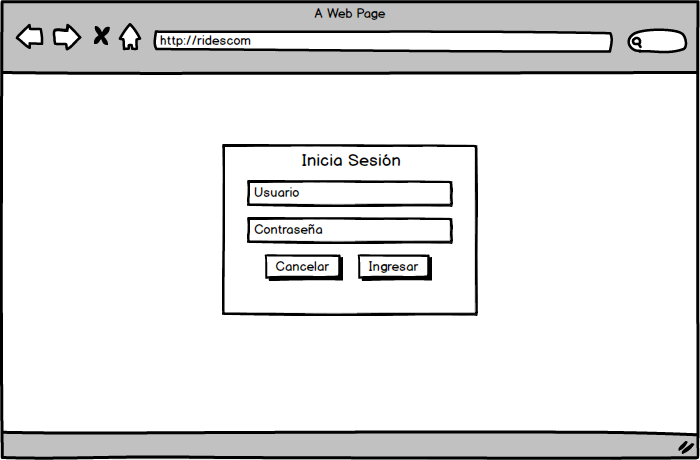
\includegraphics[width=10cm, height=6cm]{Imagenes/Nuevos/P1_LoginJFD_coord}
			\caption{Inicio sesión para el JFD y el coordinador de U.A.}
			\label{inicioJFDycoord}
		\end{figure}
		\pagebreak
		
		\begin{figure}[hbt!]
			\centering
			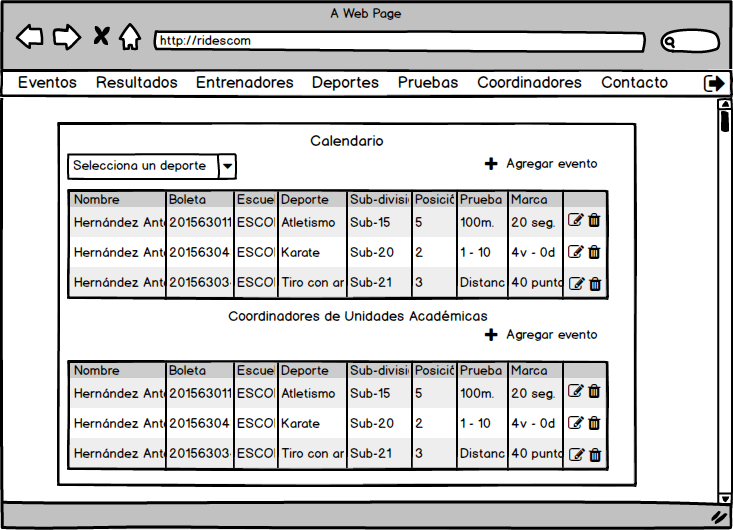
\includegraphics[width=10cm, height=6cm]{Imagenes/Nuevos/P2_Inicio_JefeFD}
			\caption{Página principal para el Jefe de Fomento Deportivo}
			\label{principalJFD}
		\end{figure}
	
		\begin{figure} [hbt!]
			\centering
			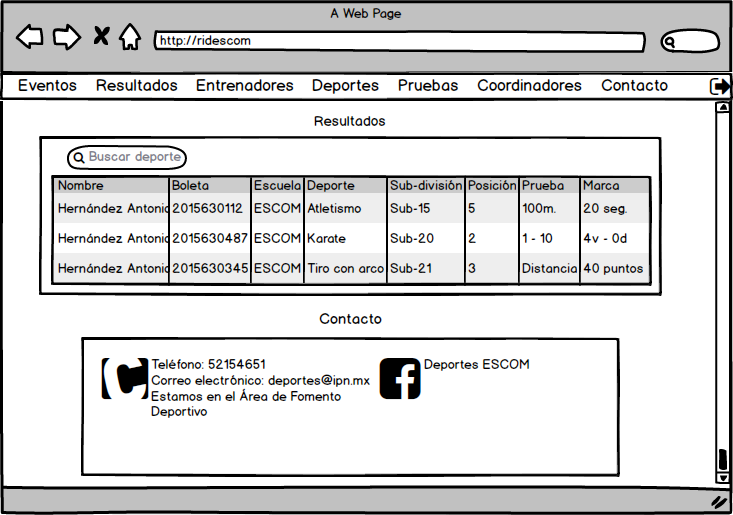
\includegraphics[width=10cm, height=6cm]{Imagenes/Nuevos/P3_Inicio_JefeFD1}
			\caption{Página principal para el Jefe de Fomento (Continuación).}
			\label{principalJFD1}
		\end{figure}
	
		\begin{figure} [hbt!]
			\centering
			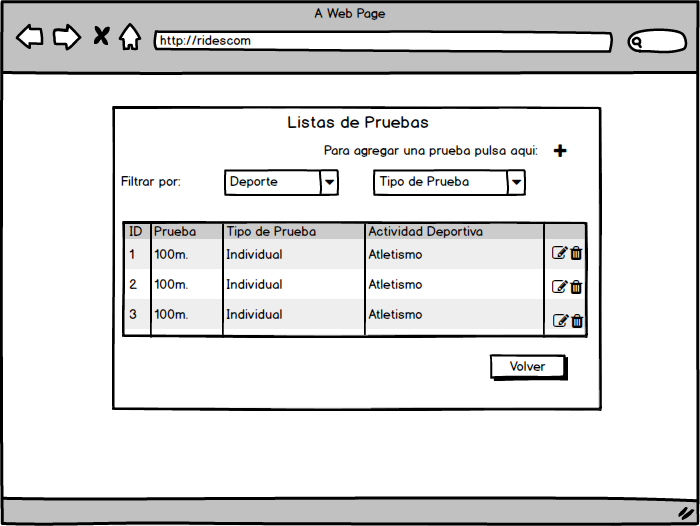
\includegraphics[width=10cm, height=6cm]{Imagenes/Nuevos/P25_Pruebas_JFD}
			\caption{Página para visualizar las pruebas dadas de alta. (Jefe de Fomento Deportivo)}
			\label{pruebas}
		\end{figure}
		\pagebreak
		
		\begin{figure} [hbt!]
			\centering
			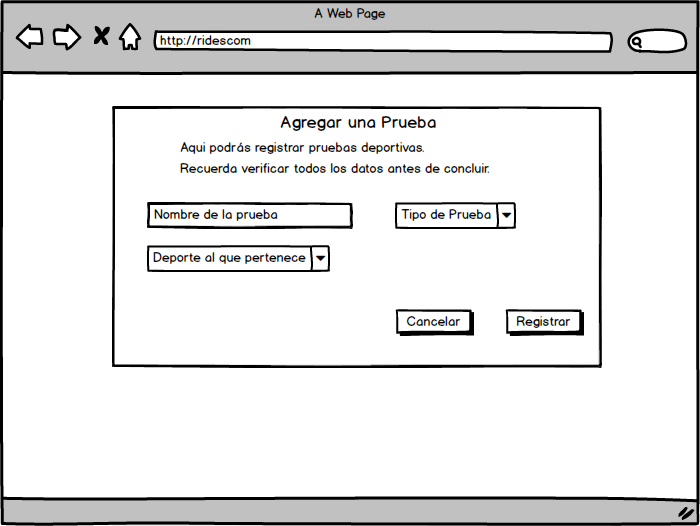
\includegraphics[width=10cm, height=6cm]{Imagenes/Nuevos/P26_AgregarPruebas_JFD}
			\caption{Página para agregar las distintas pruebas pruebas. (Jefe de Fomento Deportivo)}
			\label{agregarpruebas}
		\end{figure}
		
		\begin{figure} [hbt!]
			\centering
			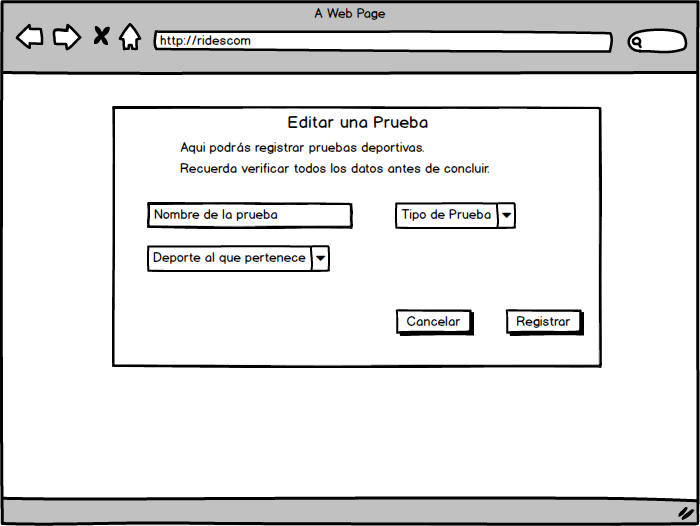
\includegraphics[width=10cm, height=6cm]{Imagenes/Nuevos/P26_EditarPruebas_JFD}
			\caption{Página para editar los datos de las pruebas previamente registrados. (Jefe de Fomento Deportivo)}
			\label{editarpruebas}
		\end{figure}
	
		\begin{figure} [hbt!]
			\centering
			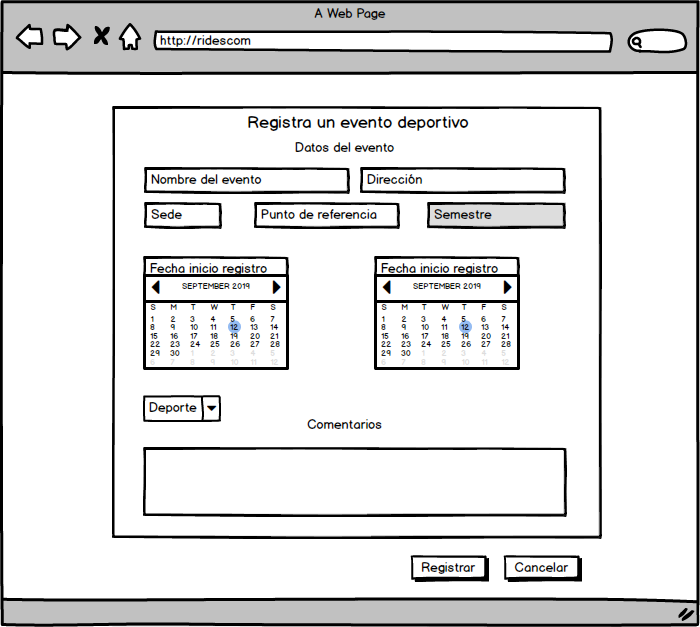
\includegraphics[width=10cm, height=6cm]{Imagenes/Nuevos/P4_Crear_evento_deportivo}
			\caption{Vista para dar de alta un evento deportivo (Jefe de Fomento Deportivo).}
			\label{creaevento}
		\end{figure}
		\pagebreak	
		
		\begin{figure} [hbt!]
			\centering
			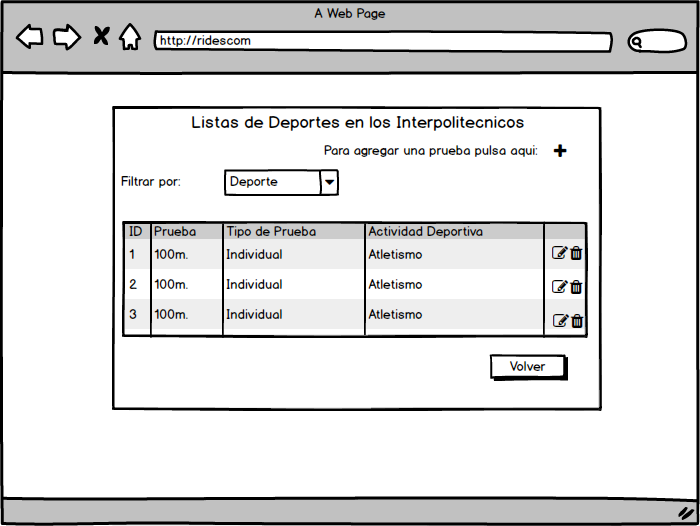
\includegraphics[width=10cm, height=6cm]{Imagenes/Nuevos/P27_Deportes_JFD}
			\caption{Página para visualizar los deportes que se llevaran a cabo en los eventos interpolitécnicos}
			\label{deportes}
		\end{figure}
	
		\begin{figure} [hbt!]
			\centering
			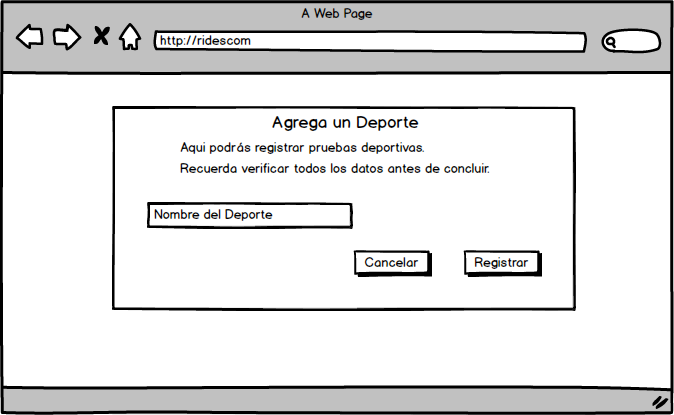
\includegraphics[width=10cm, height=6cm]{Imagenes/Nuevos/P28_AgregarDeportes_JFD}
			\caption{Página para agregar un deporte.}
			\label{agregadeporte}
		\end{figure}
		
		\begin{figure} [hbt!]
			\centering
			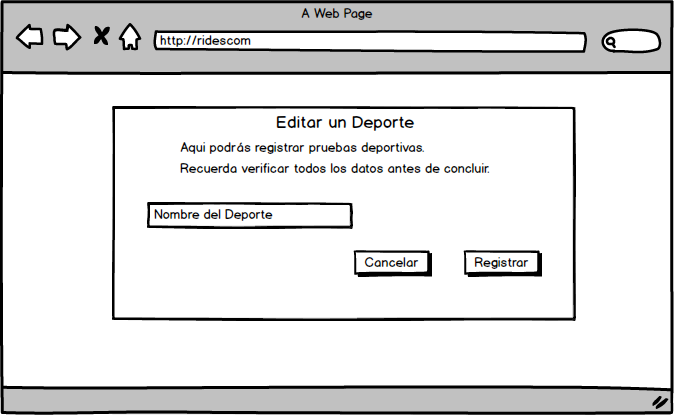
\includegraphics[width=10cm, height=6cm]{Imagenes/Nuevos/P29_EditarDeportes_JFD}
			\caption{Página para editar datos de los deportes}
			\label{editardeporte}
		\end{figure}
		\pagebreak
		
		\begin{figure} [hbt!]
			\centering
			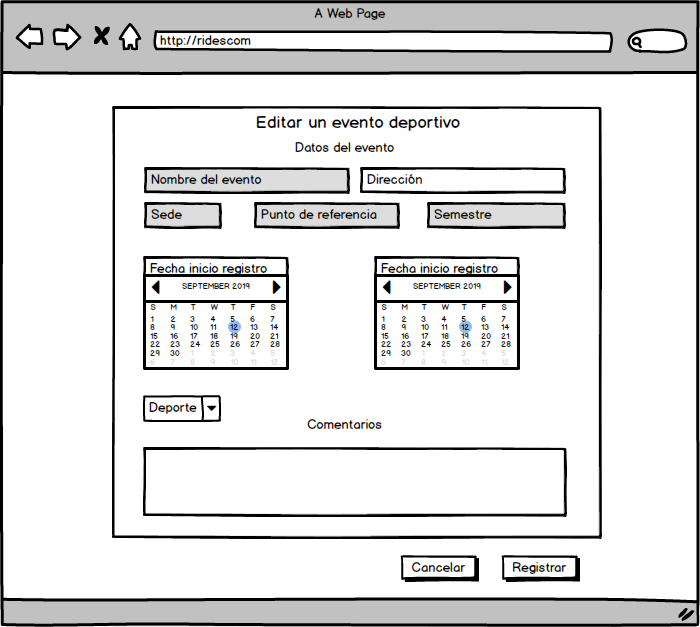
\includegraphics[width=10cm, height=6cm]{Imagenes/Nuevos/P5_Editar_evento_deportivo}
			\caption{Vista para editar datos de un evento ya registrado. (Jefe de FOmento Deportivo).}
			\label{editarevento}
		\end{figure}
	
		\begin{figure} [hbt!]
			\centering
			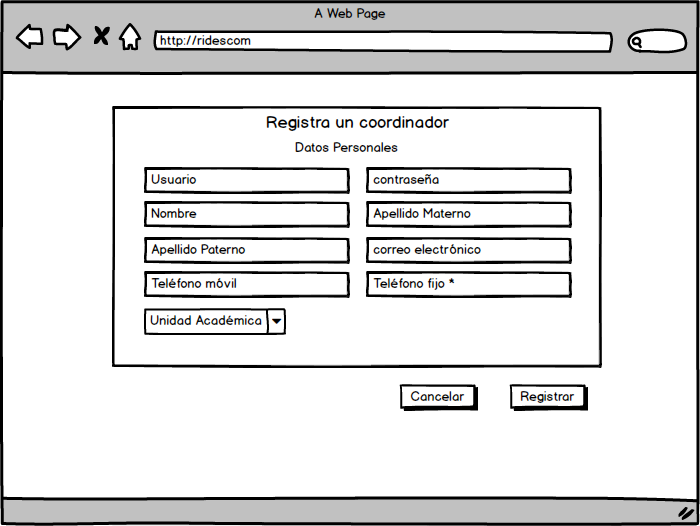
\includegraphics[width=10cm, height=6cm]{Imagenes/Nuevos/P6_Registro_coordinador}
			\caption{Vista para registrar un coordinador de unidad académica. (Jefe de Fomento Deportivo).}
			\label{registrarcoord}
		\end{figure}
		
		\begin{figure} [hbt!]
			\centering
			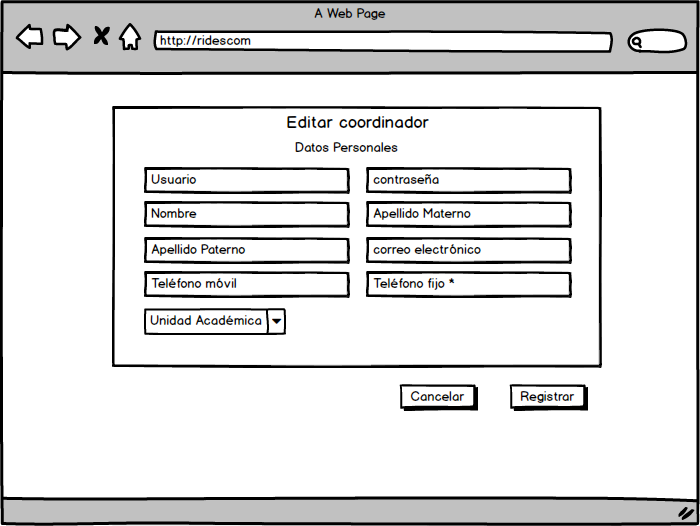
\includegraphics[width=10cm, height=6cm]{Imagenes/Nuevos/P7_Editar_coordinador}
			\caption{Vista para editar datos de un coordinador previamente registrado. (Jefe de Fomento Deportivo).}
			\label{editarcoord}
		\end{figure}
\pagebreak

		\begin{figure} [hbt!]
			\centering
			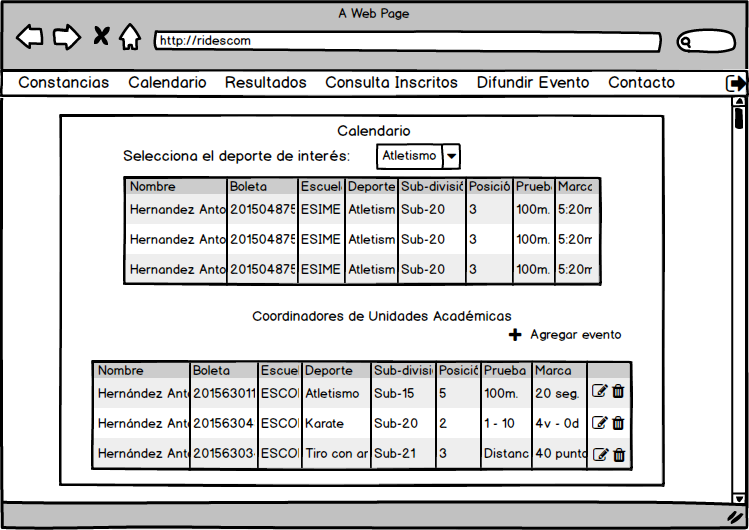
\includegraphics[width=10cm, height=6cm]{Imagenes/Nuevos/P8_Inicio_CoordUA}
			\caption{Vista principal para el coordinador de una Unidad Académica.}
			\label{principalcoord}
		\end{figure}
	
		\begin{figure} [hbt!]
			\centering
			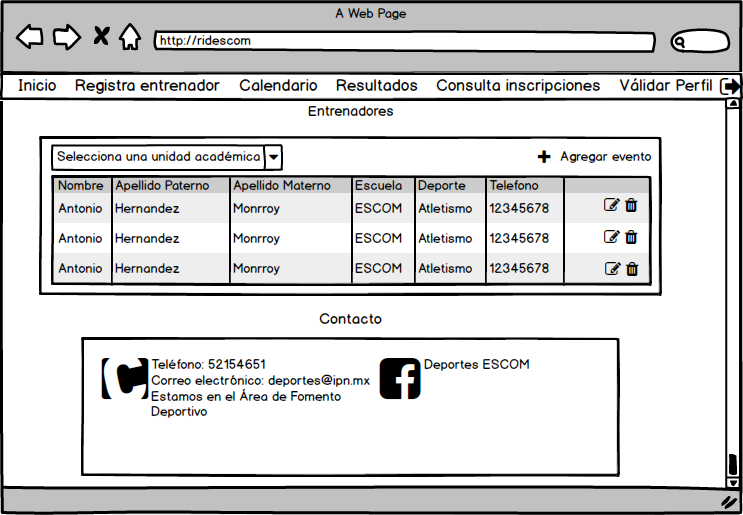
\includegraphics[width=10cm, height=6cm]{Imagenes/Nuevos/P9_Inicio_CoordUA1}
			\caption{Vista principal para el coordinador de una Unidad Académica (Continuación).}
			\label{principalcoord1}
		\end{figure}
	\pagebreak
		
		\begin{figure} [hbt!] 
			\centering
			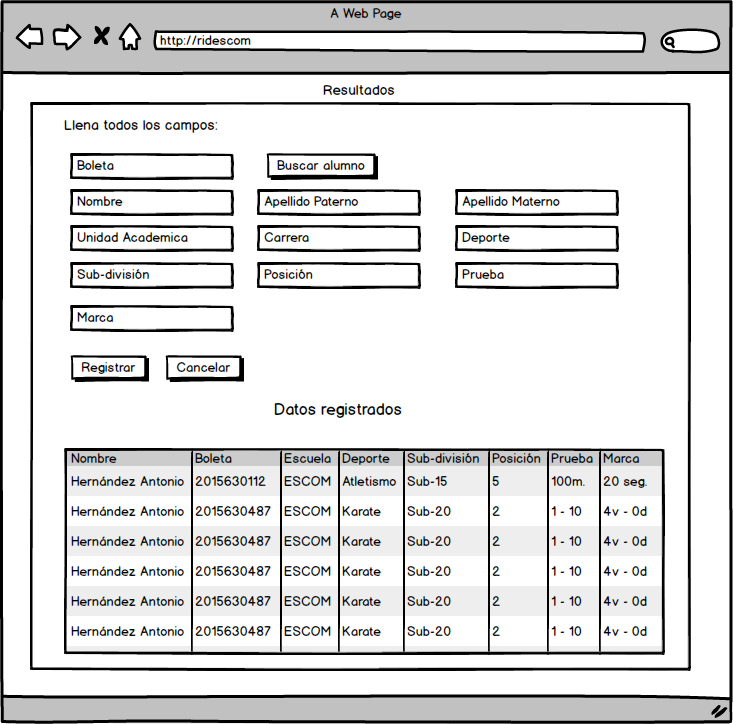
\includegraphics[width=10cm, height=7cm]{Imagenes/Nuevos/P10_Ingresa_resultados}
			\caption{Vista para ingresar los resultados obtenidos por los participantes (Coordinador de Unidad Académica).}
			\label{ingresaresultados}
		\end{figure}
		
		\begin{figure} [hbt!]
			\centering
			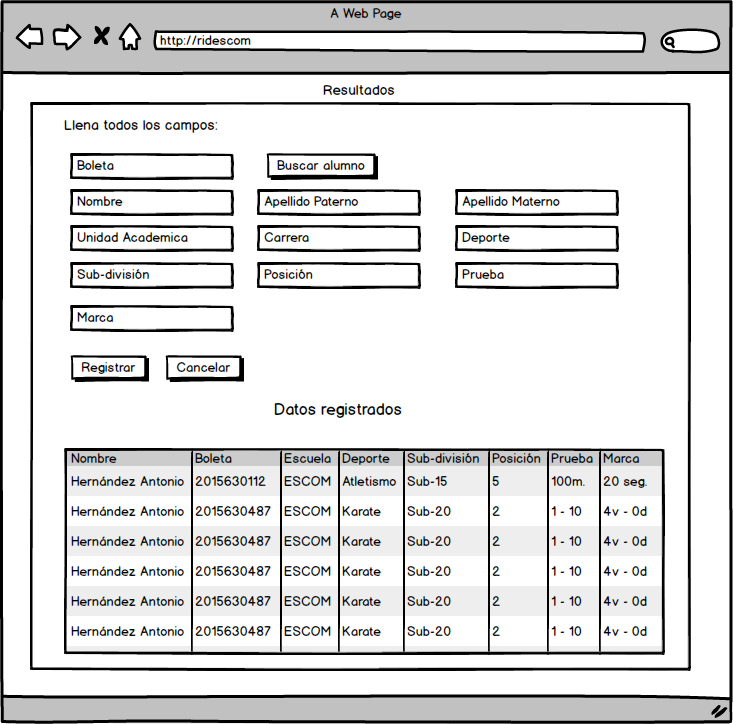
\includegraphics[width=10cm, height=7cm]{Imagenes/Nuevos/P11_Editar_resultados}
			\caption{Vista para editar los resultados de los participantes (Coordinador de Unidad Académica).}
			\label{editaresultados}
		\end{figure}
		\pagebreak
		
		\begin{figure} [hbt!]
			\centering
			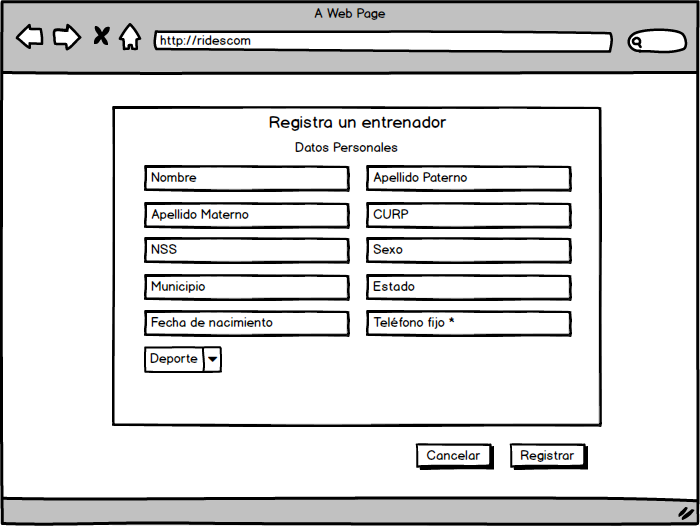
\includegraphics[width=10cm, height=6cm]{Imagenes/Nuevos/P12_Registro_entrenador}
			\caption{Vista para registrar a un entrenador (Coordinador de Unidad Académica).}
			\label{registroentrenador}
		\end{figure}
		
		\begin{figure} [hbt!]
			\centering
			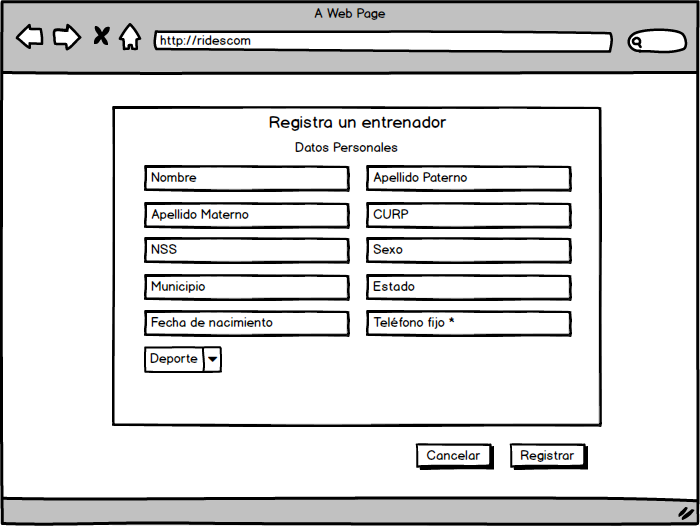
\includegraphics[width=10cm, height=6cm]{Imagenes/Nuevos/P13_Editar_entrenador}
			\caption{Vista para editar los datos del entrenador (Coordinador de Unidad Académica).}
			\label{editarentrenador}
		\end{figure}
		
		\begin{figure} [hbt!]
			\centering
			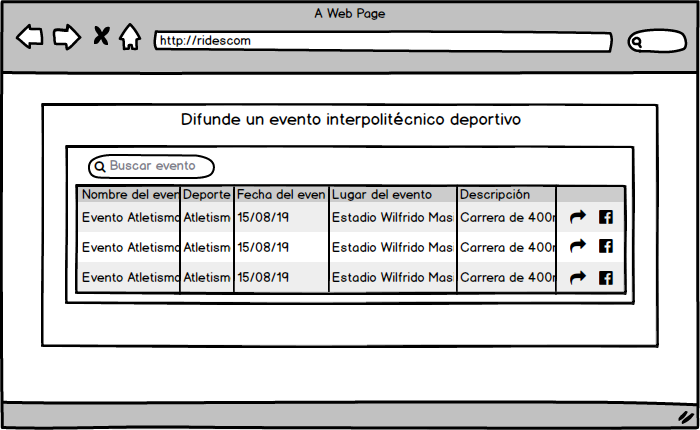
\includegraphics[width=10cm, height=6cm]{Imagenes/Nuevos/P14_Difundir_evento}
			\caption{Vista para difundir un evento interpolitécnico deportivo (Coordinador de Unidad Académica).}
			\label{difundirevento}
		\end{figure}
		\pagebreak

		\begin{figure} [hbt!]
			\centering
			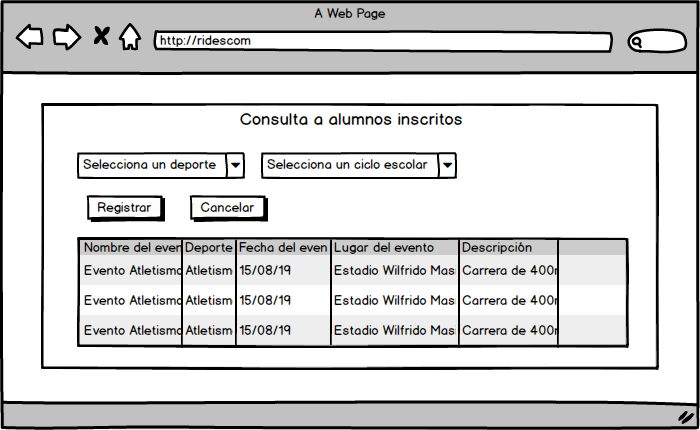
\includegraphics[width=10cm, height=6cm]{Imagenes/Nuevos/P15_Consulta_alumnos_inscritos}
			\caption{Vista para consultar los alumnos que se han inscrito a un evento (Coordinador de Unidad Académica).}
			\label{consultaalumnosinscritos}
		\end{figure}
	
		\begin{figure} [hbt!]
			\centering
			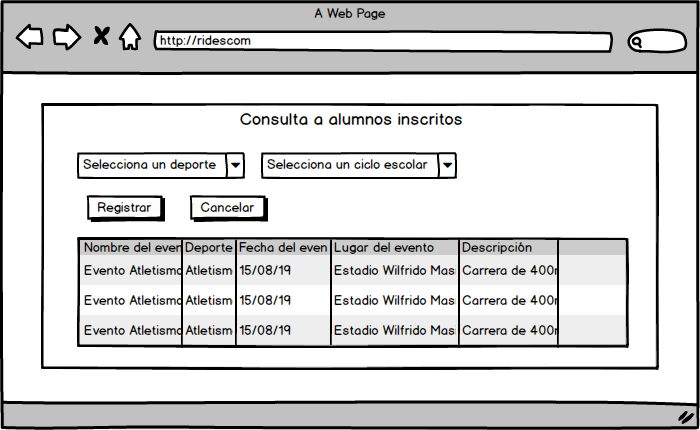
\includegraphics[width=10cm, height=6cm]{Imagenes/Nuevos/P16_Consulta_para_expedir_constancias}
			\caption{Vista para consultar participación de alumnos (Coordinador).}
			\label{consultaparaexpedirconstancias}
		\end{figure}
		
		\begin{figure} [hbt!]
			\centering
			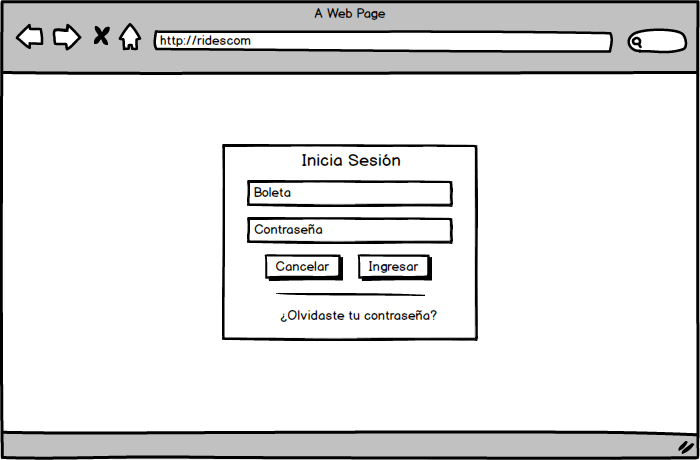
\includegraphics[width=10cm, height=6cm]{Imagenes/Nuevos/P17_Login_alumno}
			\caption{Vista Inicio de Sesión para el alumno.}
			\label{loginalumno}
		\end{figure}
	\pagebreak
		
		\begin{figure} [hbt!]
			\centering
			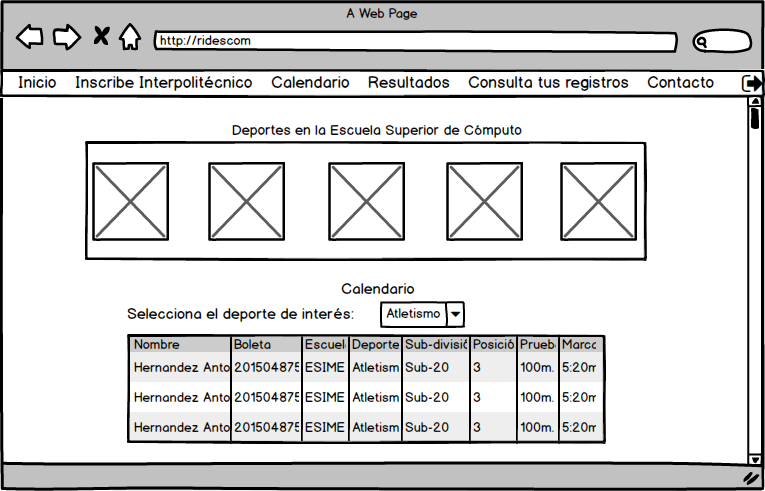
\includegraphics[width=10cm, height=6cm]{Imagenes/Nuevos/P18_Inicio_paticipante}
			\caption{Vista principal del alumno.}
			\label{principalalum}
		\end{figure}
		
		\begin{figure} [hbt!]
			\centering
			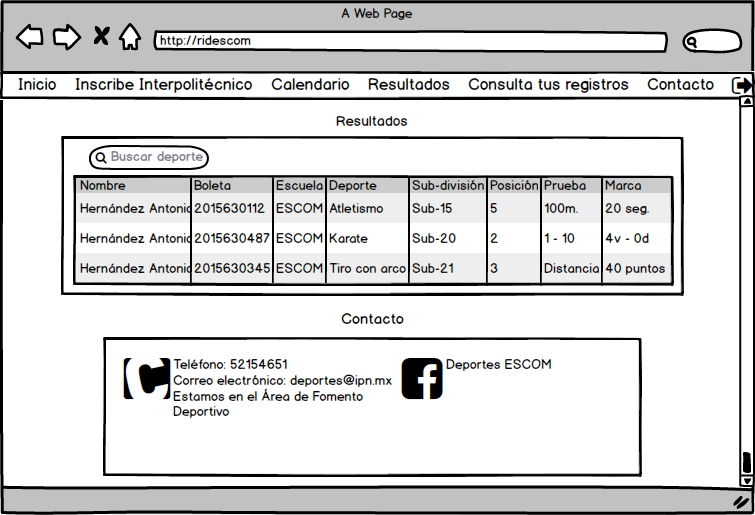
\includegraphics[width=10cm, height=6cm]{Imagenes/Nuevos/P19_Inicio_paticipante1}
			\caption{Vista principal del alumno (Continuación).}
			\label{principalalum1}
		\end{figure}
	
		\begin{figure} [hbt!]
			\centering
			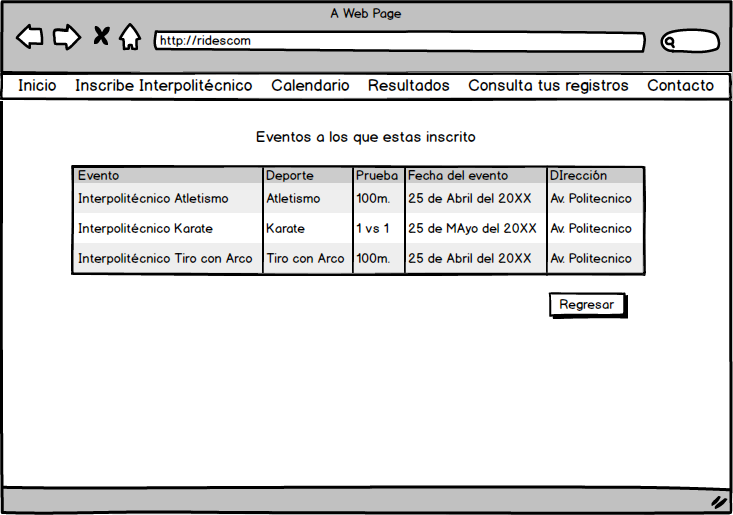
\includegraphics[width=10cm, height=6cm]{Imagenes/Nuevos/P20_Consulta_Inscripciones}
			\caption{Vista para consultar los eventos a los que se a registrado el alumno (Alumno).}
			\label{consultainscripcion}
		\end{figure}
	\pagebreak
		
		\begin{figure} [hbt!]
			\centering
			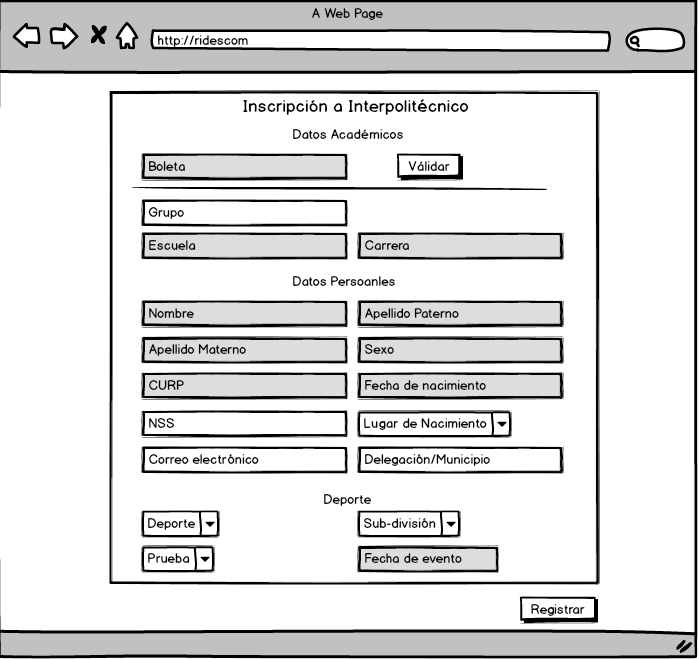
\includegraphics[width=10cm, height=6cm]{Imagenes/Disenos/Inscripcioninter}
			\caption{Formulario para que el alumno se registre en un evento interpolitécnico deportivo.}
			\label{Inscripcioninterpolitecnico}
		\end{figure}
		

		\begin{figure} [hbt!]
			\centering
			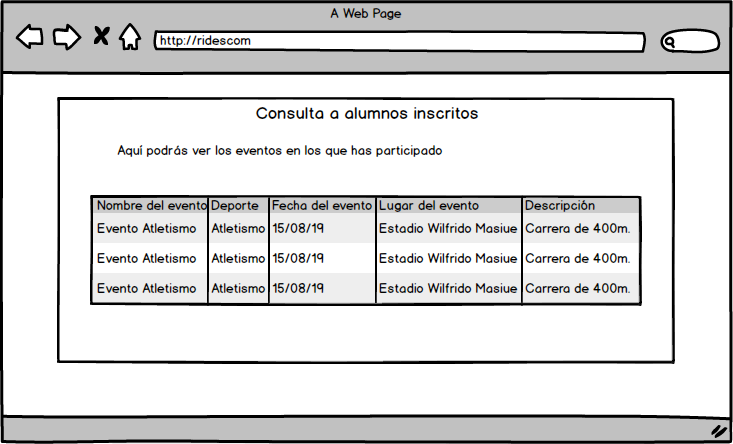
\includegraphics[width=10cm, height=6cm]{Imagenes/Nuevos/P21_Historial}
			\caption{Vista para que el alumno pueda visualizar todos los eventos en los que ha participado.}
			\label{historial}
		\end{figure}

	\chapter{Apartado C: Diagrama de Procesos}	
		\noindent Este apartado esta destinado para mostrar el diagrama del proceso actual refiriendose al proceso de inscripción a un evento interpolitécnico deportivo y a su vez, se muestra el proceso propuesto del mismo.
		
		\begin{figure}[hbt!]
			\centering
			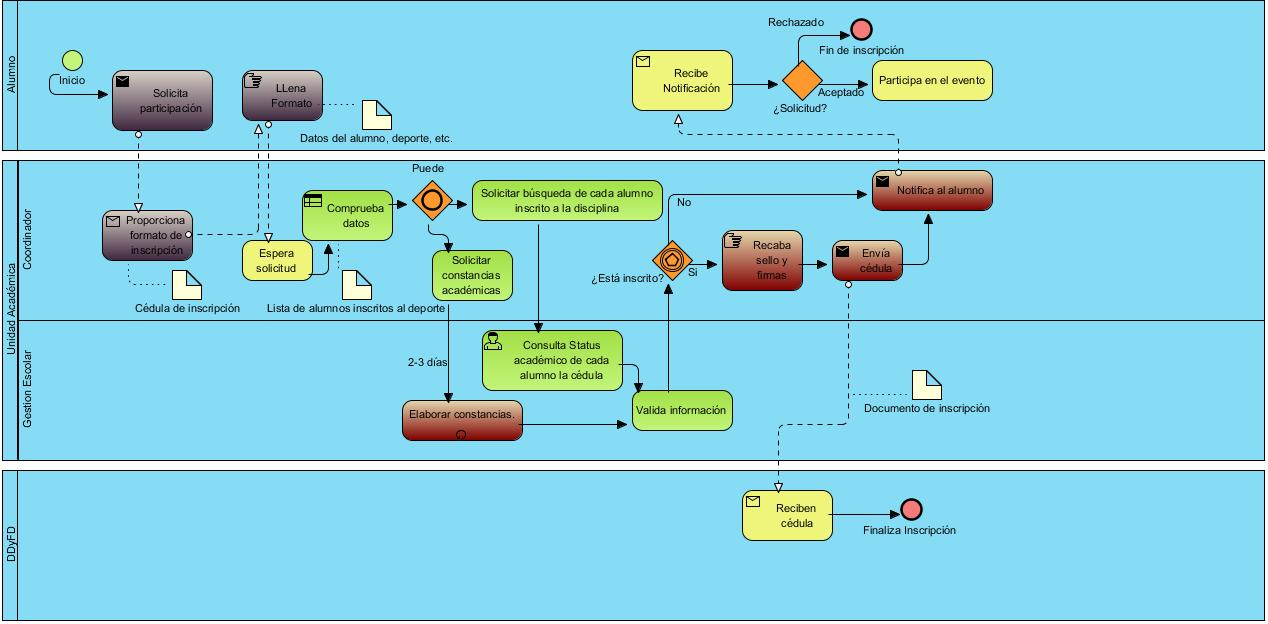
\includegraphics[width=16cm, height=8cm]{Imagenes/Disenos/ProcesoInscripcionActual.jpg}
			\caption{Proceso actual para la inscripcion a un evento interpolitécnico deportivo.}
			\label{ProcesoInscripcionActual}
		\end{figure}
	\pagebreak
	
		\begin{figure}[hbt!]
			\centering
			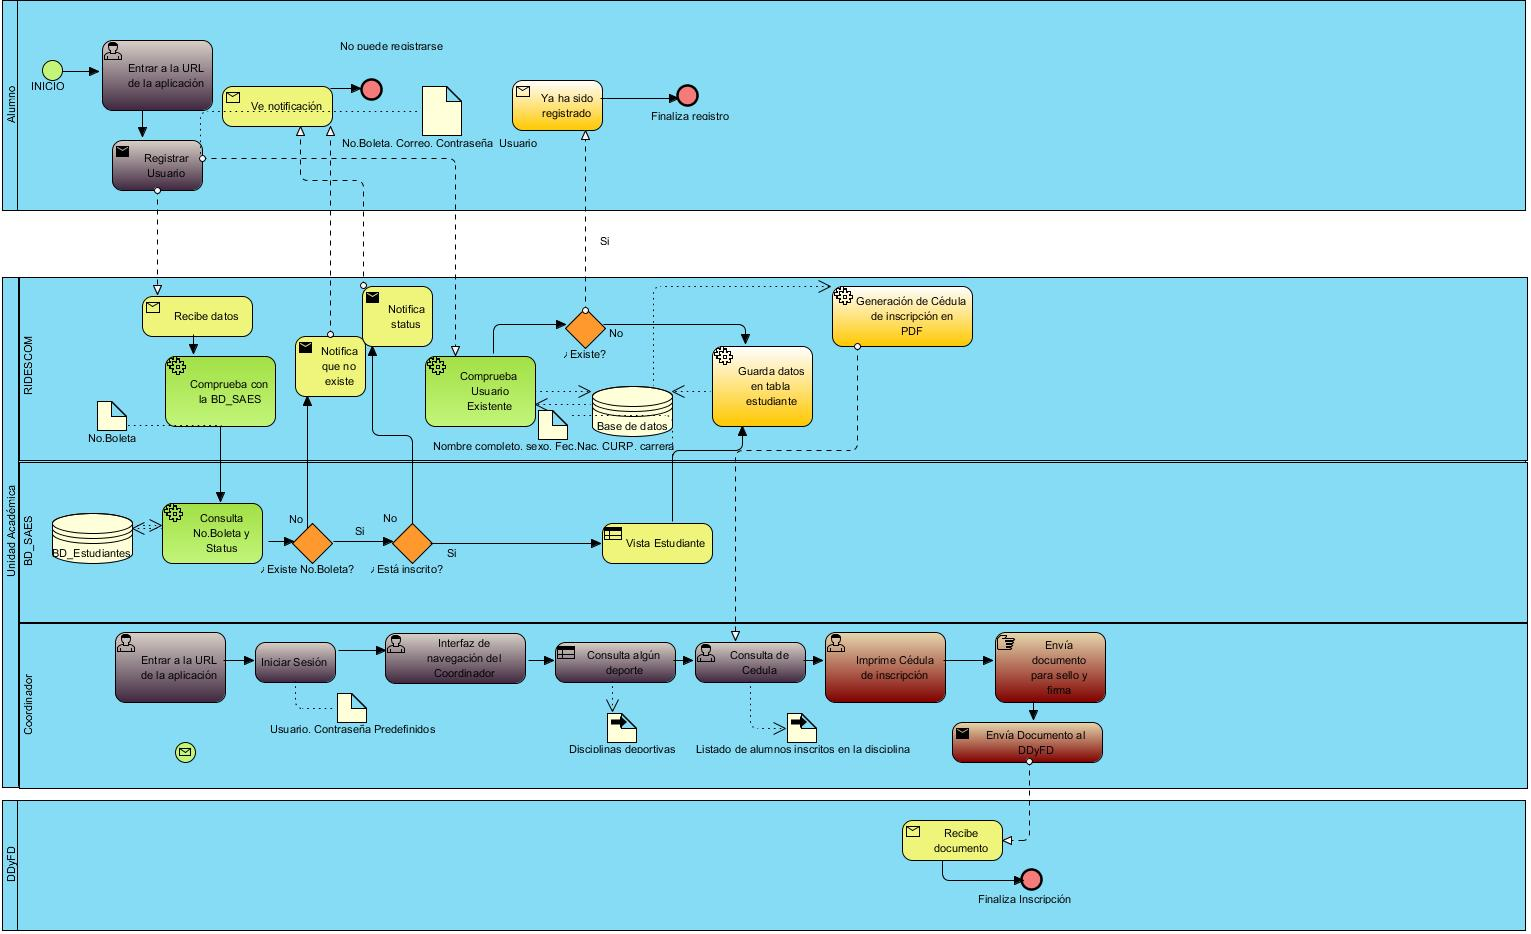
\includegraphics[width=16cm, height=8cm]{Imagenes/Disenos/ProcesoInscripcionPropuesto.jpg}
			\caption{Proceso propuesto para la inscripcion a un evento interpolitécnico deportivo.}
			\label{ProcesoInscripcionPropuesto}
		\end{figure}
	
	
	\chapter{Apartado D: Diagramas de Casos de Uso}
	\noindent En este apartado se muestra el diagrama de casos de uso de los actores, la interacción con cada uno de ellos y como funcionaria dentro de la aplicación web.
		\begin{figure}[hbt!]
			\centering
			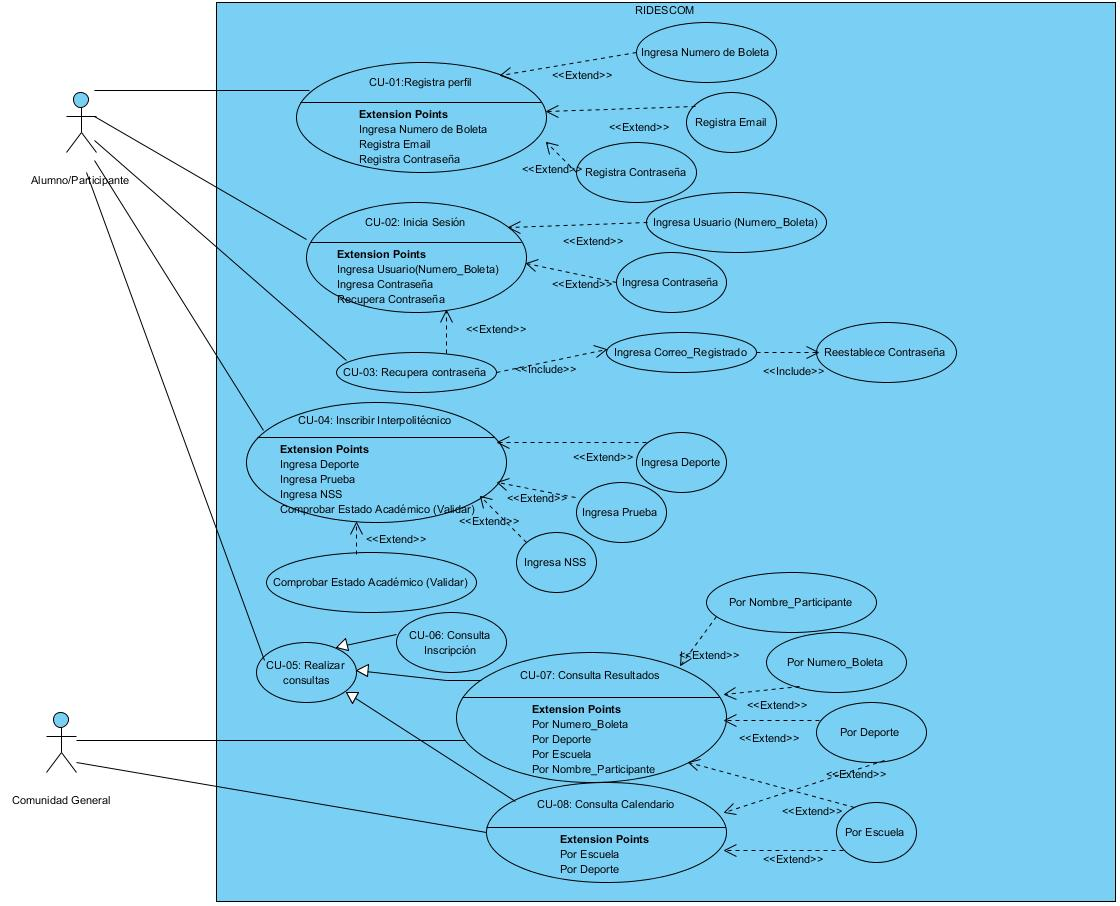
\includegraphics[width=16cm, height=8cm]{Imagenes/Disenos/DiagramasCU/Alumno.jpg}
			\caption{Diagrama de procesos Inscripción actual para un evento interpolitécnico deportivo.}
			\label{Inscripcion}
		\end{figure}
	\pagebreak
		\begin{figure}[hbt!]
			\centering
			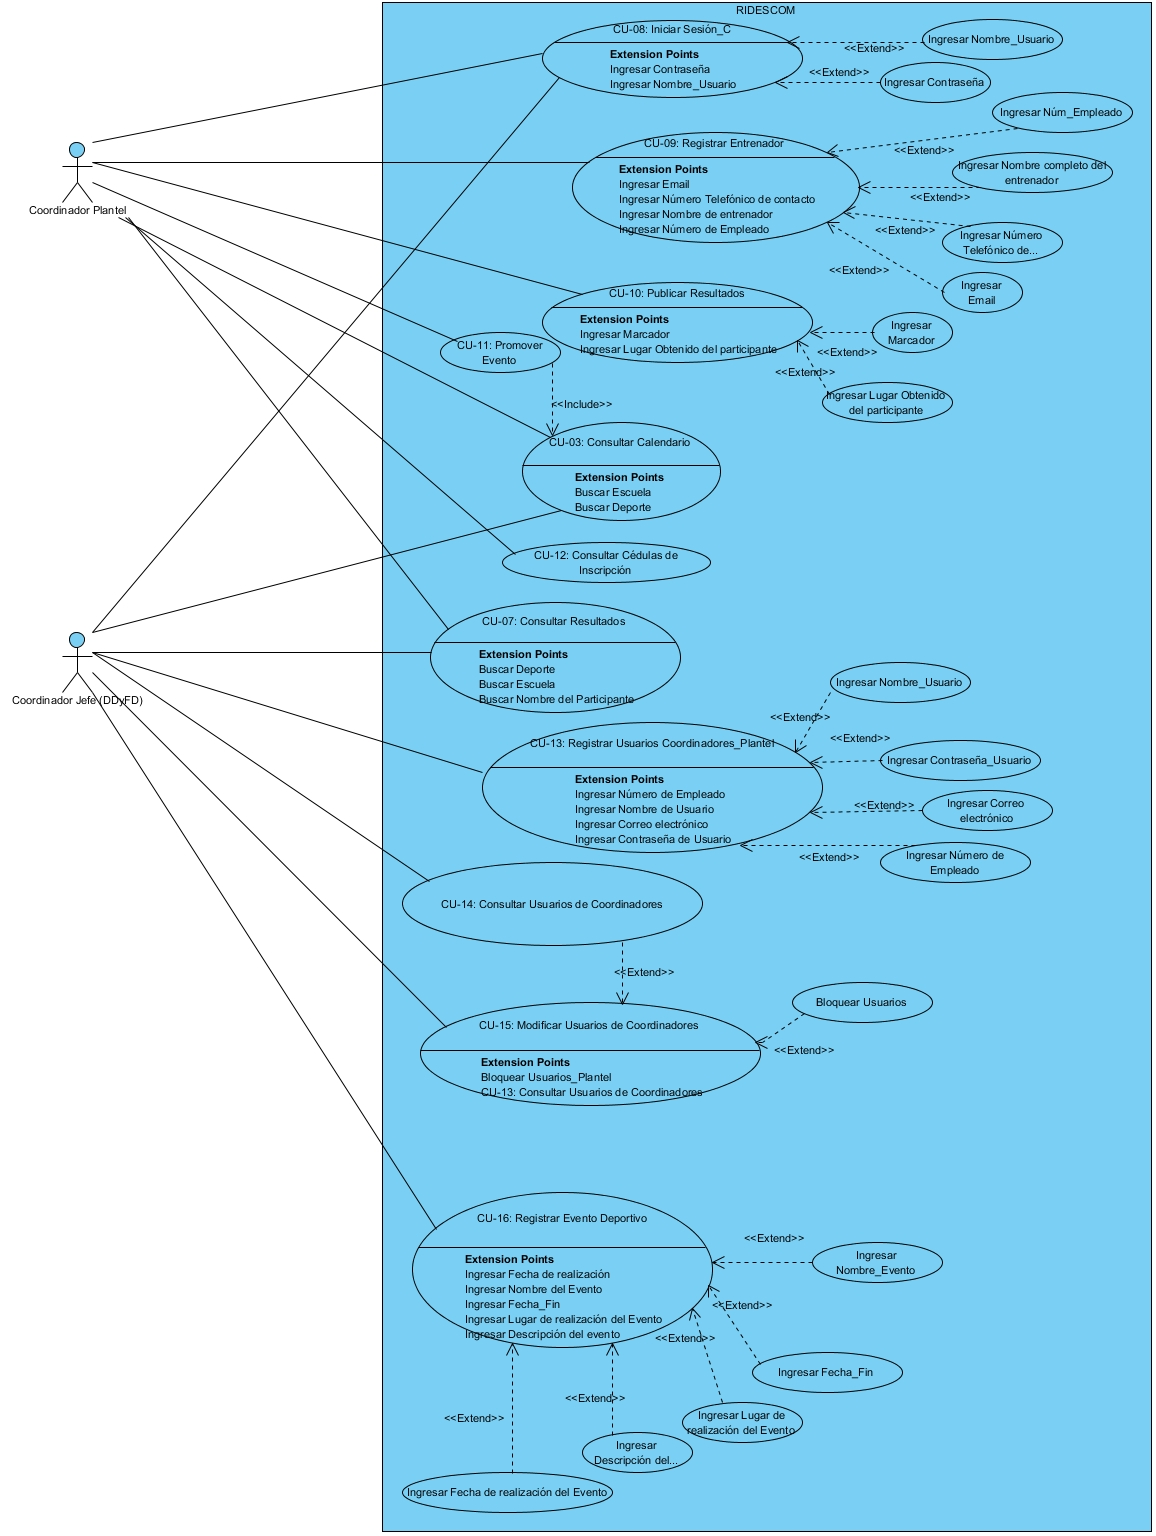
\includegraphics[width=16cm, height=12cm]{Imagenes/Disenos/DiagramasCU/CoordinadoresFinal.jpg}
			\caption{Diagrama de procesos Inscripción propuesto para un evento interpolitécnico deportivo.}
			\label{Inscripcion}
		\end{figure}
	
	\chapter{Apartado E: An\'alisis de Entornos de Desarrollo Interactivo}
	
		
		%=========================================================
		%                                                         IDE
		%=========================================================
		\section{IDE}
		\begin{itemize}
			\item  Netbeans 
			\label{Herramientas}
			\newline
			Netbeans es un entorno integrado de desarrollo o IDE (IntegratedDevelopmentEnvironment), cone el que se puede realizar todas las tareas asociadas a la programación.
			\newline
			Simplifica alguna de las tareas que, sobretodo en proyectos grandes, son laboriosas. Ofrece la posibilidad de asistencia (parcialmente) en la escritura de código, aunque no nos libera de aprender el lenguaje de programación.
			Nos ayuda en la navegación de las clases predefinidas.
			Aunque puede ser costoso su aprendizaje, los beneficios superan las dificultades.
			
			\subsection{Framework}
			\item Spring MVC \\ 
			Spring Mvc es una alternativa de framework basado en el patrón modelo-vista-controlador, después de haber aprendido de errores de frameowrks como Jakarta Struts y otras alternativas.
			El framework tiene un conjunto de interfaces que después se implementan para proporcionar la funcionalidad correspondiente. Las interfaces están acopladas claramente al Servlet Api.\cite{spring}\\
			La clase DispatcherServlet está en el front controller y es responsable de delegar y coordinar el control entre varias interfaces en la fase de ejecución durante una petición Http.
			Las interfaces más importantes definidas en Spring Mvc, y sus responsabilidades, son las siguientes:
			\begin{itemize}
				\item HandlerMapping: permite manejar peticiones de entrada.
				\item HandlerAdapter: ejecución de objetos que permiten manejar las peticiones entrantes.
				\item Controller: está entre el modelo y la vista, y permite manejar peticiones entrantes y redirigirlas a la respuesta adecuada. 
				\item Vista: responsable de retornar una respuesta al cliente. 
				\item ViewResolver: selecciona una vista basada en un nombre lógico de la vista.
				\item HandlerInterceptor: intercepta las peticiones entrantes, es comparable pero no igual a los filtros de Servlet.
				\item LocaleResolver: resuelve y opcionalmente salva el locale de un usuario individual.
				\item MultipartResolver: facilita trabajar con ficheros de subida wrapping peticiones de entrada.
			\end{itemize}
			Cada interfaz de estrategia tiene su responsabilidad importante dentro del framework general. Estas abstracciones ofrecidas por estas interfaces son potentes, pues permiten configurar un conjunto de interfaces juntas y ofrecen un conjunto en el top del Api de Servlet. Sin embargo, los desarrolladores y los vendedores son libres es escribir otras implementaciones. Spring MVC utiliza la interfaz java.util.Map como una abstracción del modelo cuando se espera que las llaves tenga valores de String. \\
			Cada testeo de las implementaciones de estas interfaces tiene otra ventaja importante dentro del alto nivel de abstracción ofrecido por Spring Mvc. Dispatcher Servlet está altamente acoplado con el contenedor de Inversión de Control de Spring para configurar las capas de web de las aplicaciones. Sin embargo, las aplicaciones web pueden utilizar otras partes del framework de Spring, incluyendo el contenedor, y decidir no usar Spring Mvc. \cite{MVC}\\
			Struts es un framework mucho más antiguo, por lo que Spring ha aprendido de la experiencia adquirida de usar Struts para no cometer los mismos errores. \cite{introspring}
			A continuación se enumeran un conjunto de ventajas:
			\begin{itemize}
				\item Spring MVC ofrece una división limpia entre Controllers, Models (JavaBeans) y Views. 
				\item Spring MVC es muy flexible, ya que implementa toda su estructura mediante interfaces, no como Struts que obliga a heredar de clases concretas tanto en sus Actions como en sus Forms. 
				\item Spring MVC provee interceptores y controllers que permiten interpretar y adaptar el comportamiento común en el manejo de múltiples requests.
				\item Los controllers de Spring MVC se configuran mediante IoC como los demás objetos, lo cual los hace fácilmente testeables e integrables con otros objetos que estén en el contexto de Spring, y por tanto sean manejables por éste. 
				\item Las partes de Spring MVC son más fácilmente testeables que las de Struts, debido a que evita la herencia de una clase de manera forzosa y una dependencia directa en el controller del servlet que despacha las peticiones. 
				\item No existen ActionForms, se enlaza directamente con los beans de negocio. 
				\item Struts obliga a extender la clase Action, mientras que Spring MVC no, aunque proporciona una serie de implementaciones de Controllers para que el usuario los utilice. Existe una gran variedad de Controladores.
				\item Spring tiene una interfaz bien definida para la capa de negocio. 
				\item Spring ofrece mejor integración con tecnologías distintas a JSP, como Velocity,XSLT,FreeMaker y XL. 
			\end{itemize}
			Las ventajas que se tiene usar Spring MVC 
			\begin{itemize}
				\item Se ha introduce un nombre es espacio MVC que simplifica la configuración.
				\item Se han insertado anotaciones adicionales como @CookieValue (permite relacionar un atributo de un método a una cookie) y @RequestMappings (asociar directamente en la clase la posibilidad de asociar una petición Url a un controlador específico).
				\item El tipo ConversionService es una alternativa más simple y robusta que los PropertyEditors de JavaBeans.
				\item Se soporta un formateo de números con el atributo @NumberFormat.
				\item Se soportan el formateo de fechas, calendarios y joda time con el atributo @DatetimeFormat, siempre que la librería Joda Time esté dentro del classpath.
				\item Se soporta la validación para entradas @Controller con la etiqueta @Valid, si se proporciona una implementación de la Jsr-303 en el classpath.
				\item Soporte para leer y escribir Xml, si Jaxb está dentro del classpath.
				\item Soporte para leer y escribir Json, si Jackson está dentor del classpath.
			\end{itemize}
			Para poder crear los controladores debemos de seguir los siguientes pasos:
			\begin{itemize}
				\item Definir una clase que implementa la interfaz del controlador.
				\item Insertar dicha clase como un objeto en el contexto de Spring.
				\item Asignar el nombre a una Uri que posteriormente será invocada por el usuario.
				\item Especificar la extensión de la uti en el DispatcherServlet de Spring, configurado en web.xml, para que se pueda buscar internamente.
			\end{itemize}
			
			El modelo son los datos con los que interactúa la vista y el controlador. En este caso, el modelo se pasa mediante un atributo de la clase ModelAndView, para posteriormente acceder al mismo desde la parte de la vista. \cite{introspring}
			
			Algunas recomendaciones para desarrollar usando Spring MVC
			Primero: determinar el Ide de desarrollo que se quiera utilizar. Existan varias alternativas: Netbeans, Eclipse, Intellij, Spring Tool Suite. Yo, por precio (gratis) y facilidad de uso (está orientado al desarrollo de Spring) recomiendo el uso de Spring Tool Suite. \\
			
			Segundo: crear el proyecto básico, y elegir nuestra herramienta de gestión de librerías. Para crear el proyecto, tenemos varias alternativas, desde configurar nosotros desde cero el servlet de spring, como utilizar plantillas ya existentes. También existe la posibilidad de descargar las librerías de la web de Spring o bien utilizar repositorios de Maven.\\
			
			Tercero: escoger el tipo de vista que se utilizará para el proyecto. En mi caso, la vista que suelo utilizar y con la que me siento más acostumbrado es Jsp.\\
			
			Cuarto: desarrollar la parte de negocio (controladores) y persistencia (seleccionando un framework como hibernate o jpa), y relacionar los controladores, con la vista y la persistencia.
			En principio, eso es todo.\\
			El framework fue lanzado inicialmente bajo Apache 2.0 License en junio de 2003. Esta licencia es una licencia de software libre creada por la Apache Software Foundation que requiere la conservación del aviso de copyright y disclaimer, pero no es una liencia copyleft, ya que no requiere la redistribución del código fuente cuando se distribuyen versiones modificadas. \cite{introspring} \\
			
			\item Facebook Developers 
			La Plataforma de Facebook es el conjunto de servicios, herramientas y productos proporcionados por el servicio de redes sociales Facebook para que los desarrolladores externos creen sus propias aplicaciones y servicios que acceden a datos en Facebook.\\
			
			La actual Plataforma de Facebook se lanzó en 2010. La plataforma ofrece un conjunto de interfaces y herramientas de programación que permiten a los desarrolladores integrarse con el "gráfico social" abierto de relaciones personales y otras cosas como canciones, lugares y páginas de Facebook. La asignación en facebook.com, sitios web externos y dispositivos pueden acceder al gráfico. \\
			
			Facebook lanzó la Plataforma de Facebook el 24 de mayo de 2007, proporcionando un marco para que los desarrolladores de software creen aplicaciones que interactúen con las funciones principales de Facebook. Se introdujo un lenguaje de marcado llamado Facebook Markup Language simultáneamente; se utiliza para personalizar el "aspecto y la sensación" de las aplicaciones que crean los desarrolladores. Usando la Plataforma, Facebook lanzó varias aplicaciones nuevas, incluyendo Regalos, permitiendo a los usuarios enviarse regalos virtuales entre sí, Marketplace, permitiendo a los usuarios publicar anuncios clasificados gratuitos, eventos de Facebook, brindando a los usuarios un método para informar a sus amigos sobre los próximos eventos, Video, Permitir a los usuarios compartir videos caseros entre ellos y juegos de redes sociales, donde los usuarios pueden usar sus conexiones con amigos para ayudarlos a avanzar en los juegos que están jugando. Muchos de los primeros juegos populares de redes sociales combinarían capacidades. Por ejemplo, uno de los primeros juegos en llegar al primer lugar de aplicación, (Lil) Green Patch, combina regalos virtuales con notificaciones de eventos a amigos y contribuciones a organizaciones benéficas a través de causas. \\
			
			Componentes de plataforma de alto nivel
			API de gráficos\\
			Graph API es el núcleo de la plataforma de Facebook, lo que permite a los desarrolladores leer y escribir datos en Facebook. Graph API presenta una vista simple y coherente del gráfico social de Facebook, que representa de manera uniforme los objetos en el gráfico (por ejemplo, personas, fotos, eventos y páginas) y las conexiones entre ellos (por ejemplo, relaciones de amigos, contenido compartido y etiquetas de fotos )\\
			
			Autenticación\\
			La autenticación de Facebook permite que las aplicaciones de los desarrolladores interactúen con la API Graph en nombre de los usuarios de Facebook, y proporciona un mecanismo de inicio de sesión único en aplicaciones web, móviles y de escritorio.\\
			
			Complementos sociales\\
			Los complementos sociales, incluidos el botón Me gusta, las recomendaciones y el feed de actividades, permiten a los desarrolladores proporcionar experiencias sociales a sus usuarios con solo unas pocas líneas de HTML. Todos los complementos sociales son extensiones de Facebook y están diseñados para que no se compartan datos de los usuarios con los sitios en los que aparecen. Por otro lado, los complementos sociales permiten a Facebook rastrear los hábitos de navegación de sus usuarios a través de cualquier sitio que cuente con los complementos. Y los datos recopilados de los hábitos de navegación de los usuarios ayudan a los vendedores y anunciantes en Facebook a dirigirse a su audiencia.\\
			
			iframes\\
			Facebook usa iframes para permitir que los desarrolladores externos creen aplicaciones que están alojadas por separado de Facebook, pero operan dentro de una sesión de Facebook y se accede a través del perfil de un usuario. Dado que los iframes esencialmente anidan sitios web independientes dentro de una sesión de Facebook, su contenido es distinto del formato de Facebook. \\
			
			Originalmente, Facebook utilizaba el 'Lenguaje de marcado de Facebook (FBML)' para permitir a los desarrolladores de aplicaciones de Facebook personalizar el "aspecto y la sensación" de sus aplicaciones, hasta cierto punto. FBML es una especificación de cómo codificar contenido para que los servidores de Facebook puedan leerlo y publicarlo, lo cual es necesario en el feed específico de Facebook para que el sistema de Facebook pueda analizar el contenido y publicarlo como se especifica. Facebook almacena en caché el FBML establecido por cualquier aplicación hasta que una llamada API posterior lo reemplace. Facebook también ofrece una biblioteca especializada de JavaScript de Facebook (FBJS).\\
			
			Facebook dejó de aceptar nuevas aplicaciones FBML el 18 de marzo de 2011, pero continuó admitiendo las pestañas y aplicaciones FBML existentes. Desde el 1 de enero de 2012, FBML ya no era compatible, y FBML ya no funcionaba a partir del 1 de junio de 2012. 
		\end{itemize}
		
		
		\section{Rastreo Web y API's}
		\begin{itemize}
			\item Web Crawler\newline
			Un Web Crawler (también llamado Web Spider) es un programa diseñado para explorar páginas Web en forma automática. La operación normal es que se le da al programa un grupo de direcciones iniciales, el crawler descarga estas direcciones, analiza las páginas y busca enlaces a páginas nuevas. Luego descarga estas páginas nuevas, analiza sus enlaces, y así sucesivamente.\cite{crawling} \\
			Los crawlers se pueden usar para varias cosas, lo más común es que se usen para:
			\begin{itemize}
				\item Crear el índice de una [article-1056.html máquina de búsqueda]. 
				\item Analizar los enlaces de un sitio para buscar links rotos. 
				\item Recolectar información de un cierto tipo, como precios de productos para armar un catálogo. \cite{craw}
			\end{itemize} 
			
			Un Web Crawler es un pequeño programa que recorre permanentemente el entramado de contenidos que conforman la Red. Su principal utilidad se la otorgan los buscadores al emplearlos para rastrear nuevas webs, de las que descargan automáticamente una copia que almacenan en un índice; una vez integradas en estas bases de datos las webs podrán ser rápidamente localizadas en la siguiente consulta efectuada por los usuarios, permitiendo mostrárselas entre la lista de resultados.
			Una araña web inicia su trabajo visitando un conjunto de direcciones predeterminadas, analiza las páginas, identifica los enlaces externos que éstas puedan incluir y los añade a la lista de direcciones a visitar, perpetuándose en su labor.	\cite{web} \\
			
			Ahora bien, un rastreador web, indexador web, indizador web o araña web es un programa informático que inspecciona las páginas del World Wide Web de forma metódica y automatizada.1 Uno de los usos más frecuentes que se les da consiste en crear una copia de todas las páginas web visitadas para su procesado posterior por un motor de búsqueda que indexa las páginas proporcionando un sistema de búsquedas rápido. Las arañas web suelen ser bots. \cite{araña} \\
			
			Web scraping es una técnica utilizada mediante programas de software para extraer información de sitios web. Usualmente, estos programas simulan la navegación de un humano en la World Wide Web ya sea utilizando el protocolo HTTP manualmente, o incrustando un navegador en una aplicación.  \\
			El web scraping está muy relacionado con la indexación de la web, la cual indexa la información de la web utilizando un robot y es una técnica universal adoptada por la mayoría de los motores de búsqueda. Sin embargo, el web scraping se enfoca más en la transformación de datos sin estructura en la web (como el formato HTML) en datos estructurados que pueden ser almacenados y analizados en una base de datos central, en una hoja de cálculo o en alguna otra fuente de almacenamiento. Alguno de los usos del web scraping son la comparación de precios en tiendas, la monitorización de datos relacionados con el clima de cierta región, la detección de cambios en sitios webs y la integración de datos en sitios webs.	\cite{araña} \\
			
			El web scraping es una técnica que sirve para extraer información de páginas web de forma automatizada. Si traducimos del inglés su significado vendría a significar algo así como “escarbar una web”. \\
			Aplicaciones y ejemplos:\\
			Su uso está muy claro: podemos aprovechar el web scraping para conseguir cantidades industriales de información (Big data) sin teclear una sola palabra. A través de los algoritmos de búsqueda podemos rastrear centenares de webs para extraer sólo aquella información que necesitamos.\\
			Para ello nos será muy útil dominar regex (regular expression) para delimitar las búsquedas o hacerlas más precisas y que el filtrado de la información sea mejor.\\
			Algunos ejemplos para los cuales vamos a necesitar el web scraping:
			\begin{itemize}
				\item Para marketing de contenidos: podemos diseñar un robot que haga un ‘scrapeo’ de datos concretos de una web y los podamos utilizar para generar nuestro propio contenido. Ejemplo: scrapear los datos estadísticos la web oficial de una liga de fútbol para generar nuestra propia base de datos.
				\item Para ganar visibilidad en redes sociales: podemos utilizar los datos de un scrapeo para interactuar a través de un robot con usuarios en redes sociales. Ejemplo: crear un bot en instagram que seleccione los links de cada foto y luego programar un comentario en cada entrada.
				\item Para controlar la imagen y la visibilidad de nuestra marca en internet: a través de un scrapeo podemos automatizar la posición por la que varios artículos de nuestra web se posicionan en Google o, por ejemplo, controlar la presencia del nombre de nuestra marca en determinados foros. Ejemplo: rastrear la posición en Google de todas las entradas de nuestro blog.
			\end{itemize}	
			
			
			Para poder desarrollar un web scraping de la mejor manera se debe considerar  dos vertientes muy diferenciadas del conocimiento web, ambas esenciales para tener perfil versátil en la red. Por un lugar debemos dominar la visualización de datos a nivel conceptual y por el otro debemos disponer de los conocimientos técnicos necesarios para lograr extraer con exactitud los datos con herramientas especializadas. \\
			Al fin y al cabo esto se resumirá en saber gestionar grandes cantidades de datos (big data). Debemos estar mínimamente familiarizados con la visualización de grandes cantidades de datos con tal de poder jerarquizar e interpretar los datos que extraigamos de una web. Y no solo para extraer los datos, también a la hora de plantear la estrategia de extracción debemos saber cuales van a ser los datos que vayamos a extraer con tal de poder darles un sentido informativo para el usuario \cite{scraping}.\\
			
			\textbf{Api's más utilizadas}
			\begin{itemize}
				\item \textbf{Jsoup}: Es una libreria de Java para trabajar con HTML real en el mundo real. Proporciona una API muy conveniente para extraer y manipular datos, utilizando lo mejor de DOM, CSS y métodos similares a jquery.\\
				
				Implementa la especificación HTML5 WHATWG y analiza HTML en el mismo DOM que los navegadores modernos.
				\begin{itemize}
					\item 
					\item Raspa y analiza HTML desde una URL, archivo o cadena
					\item Encuentra y extrae datos, usando DOM transversal o selectores de CSS
					manipular los elementos HTML, atributos y texto
					\item Limpia el contenido enviado por el usuario contra una lista blanca segura, para evitar ataques XSS
					\item HTML ordenado de salida
				\end{itemize}
				
				Jsoup está diseñado para tratar con todas las variedades de HTML que se encuentran en la naturaleza; de lo prístino y de la validación para invalidar la etiqueta soup; jsoup creará un árbol de análisis sensible.\\
				
				Jsoup es un proyecto de código abierto distribuido bajo la licencia liberal MIT. El código fuente está disponible en GitHub.\cite{jsoup}
				
				\item \textbf{Selenium}: Es un automatizador de navegadores. Principalmente, es para automatizar aplicaciones web con fines de prueba, pero ciertamente no se limita a eso. Las tareas de administración aburridas basadas en la web pueden (y deberían) ser automatizadas también.\\
				
				Selenium tiene el soporte de algunos de los proveedores más grandes de navegadores que han tomado (o están tomando) pasos para hacer de Selenium una parte nativa de su navegador. También es la tecnología central en muchas otras herramientas de automatización del navegador, API y marcos.\\
				
				Selenium provee una herramienta de grabar o reproducir para crear pruebas sin usar un lenguaje de scripting para pruebas (Selenium IDE). Incluye también un lenguaje específico de dominio para pruebas (Selanese) para escribir pruebas en un amplio número de lenguajes de programación populares incluyendo Java, C$\#$, Ruby, Groovy, Perl, Php y Python. Las pruebas pueden ejecutarse entonces usando la mayoría de los navegadores web modernos en diferentes sistemas operativos como Windows, Linux y OSX.
				
			\end{itemize}
			Como Api seleccionada para trepar páginas web Jsoup es apta para la realización del trabajo ya que nos permite analizar libremente el DOM de alguna página y es mucho más rápido que selenium, ya que no necesita molestarse con un DOM "vivo". Selenium siempre debe verificar si los manejadores de elementos siguen siendo válidos antes de realizar cualquier operación con ellos pero la sobrecarga es realmente notable cuando realiza un raspado serio. \\
			
		\end{itemize}
		
		
		%=========================================================
		%                                                         Sistema Gestor de BD
		%=========================================================
		%\section{Sistema Gestor de Base de Datos}
		%\noindent Realizando una investigación de los distintos gestores de Bases de Datos encontramos las siguientes caracteristicas:
		%\begin{table}[htbp]
		%	\begin{center}
		%		\begin{tabular}{|l|p{35mm}|p{35mm}|p{35mm}|l}
		%			\hline
		%			Caracter\'isticas & Oracle & MySQL & SQL Server \\
		%			\hline 
		%			Interfaz & GUI, SQL & SQL & GUI, SQL \\ \hline
		%			Lenguaje soportado & C, C++, C, Java, Ruby y Objective-C & C, C, C++, D, Java, Ruby y Objective C & Java, Ruby, Python, VB, .Net y PHP  \\ \hline
		%			Sistema Operativo & Windows, GNU/Linux, Solaris, OS-X & Windows, GNU/Linux, OS-X, FreeBSD, Solaris & Windows \\ \hline
		%			Licencia & Propietrio & Código Libre & Propietario \\ \hline
		%		\end{tabular}
		%		\caption{Tabla comparativa de lenguajes de BD.}
		%		\label{tabla:sencilla}
		%	\end{center}
		%\end{table}
		
		\section{iReport}
		\noindent IReport. Es una herramienta visual que sirve para generar ficheros XML (plantillas de informes) utilizando la herramienta de generación de informes JasperReport.\\
		\noindent Escrito en Java IReport provee a los usuarios de JasperReport una interfaz visual para construir reportes. También permite que los usuarios corrijan visualmente informes complejos con cartas, imágenes y subinformes. \\
		Bibliotecas gráficas que emplea \\
		\noindent Está además integrado con JFreeChart, una de la bibliotecas gráficas OpenSource más difundida para Java. Los datos para imprimir pueden ser recuperados por varios caminos incluso múltiples uniones JDBC, TableModels, JavaBeans, XML, etc. \\
		
		\textbf{Características de IReport}
		La lista siguiente describe algunas de las características importantes de IReport:
		\begin{itemize}
			\item 100 porciento escrito en Java y además OpenSource y gratuito.
			\item Maneja el 98 porciento de las etiquetas de JasperReport.
			\item Permite diseñar con sus propias herramientas: rectángulos, líneas, elipses, campos de los textfields, cartas, subreports (subreportes).
			\item Soporta internacionalización nativamente.
			\item Browser de la estructura del documento.
			\item Recopilador y exportador integrados .
			\item Soporta JDBC.
			\item Soporta JavaBeans como orígenes de datos (éstos deben implementar la interface JRDataSource).
			\item Incluye Wizard’s (asistentes) para crear automáticamente informes.
			\item Tiene asistentes para generar los subreportes.
			\item Tiene asistentes para las plantillas.
			\item Facilidad de instalación.
		\end{itemize}
		
		\textbf{Requerimientos de instalación}
		\begin{itemize}
			\item Sun JDK 1.4 (SDK) o superior.
			\item Acrobat 5.0 no es requerido, pero es fuertemente recomendado.
			\item Si se desea conectar con una base de datos, se debe proporcionar el DriverJDBC correspondiente.
			\item Usar la versión IReport-0.5.1 o superior.
		\end{itemize}
		
		\textbf{Librerias que utiliza}
		\begin{itemize}
			\item jasperreports-1.0.1.jar
			\item commons-digester.jar
			\item commons-beanutils.jar
			\item commons-collections.jar
			\item commons-logging.jar
			\item itext-1.02b.jar
			\item poi-2.0-final-20040126.jar
		\end{itemize}

	\chapter{Apartado F: API Facebook}
	\label{apiFB}
	\noindent En este apartado, se menciona detalladamente la función e implementación al proyecto. Así como lo desarrollado y la problemática que se tuvo al final de la presentación del proyecto.\\
		
	\noindent Durante el periodo de pruebas realizado en Trabajo Terminal 2 nos percatamos que el módulo de difusión de eventos, no funcionaba de la manera correcta, por lo cual se realizó una revisión de este. Siendo así, nos percatamos que los terminos de uso de las herramientas de Facebook solicitaban una revisión de datos para que estás puedan ser empleadas en el proyecto, como se puede apreciar en la figura a continuación.
	
	Dentro de la investigacion se encontró que se  tenía que seguir paso a pasola verificación del negoncio y la revisión de la aplicación, con la finalidad de si está todo en orden se pueda utilizar las herramientas de Facebook.
	
	\begin{figure}[hbt!]
		\centering
		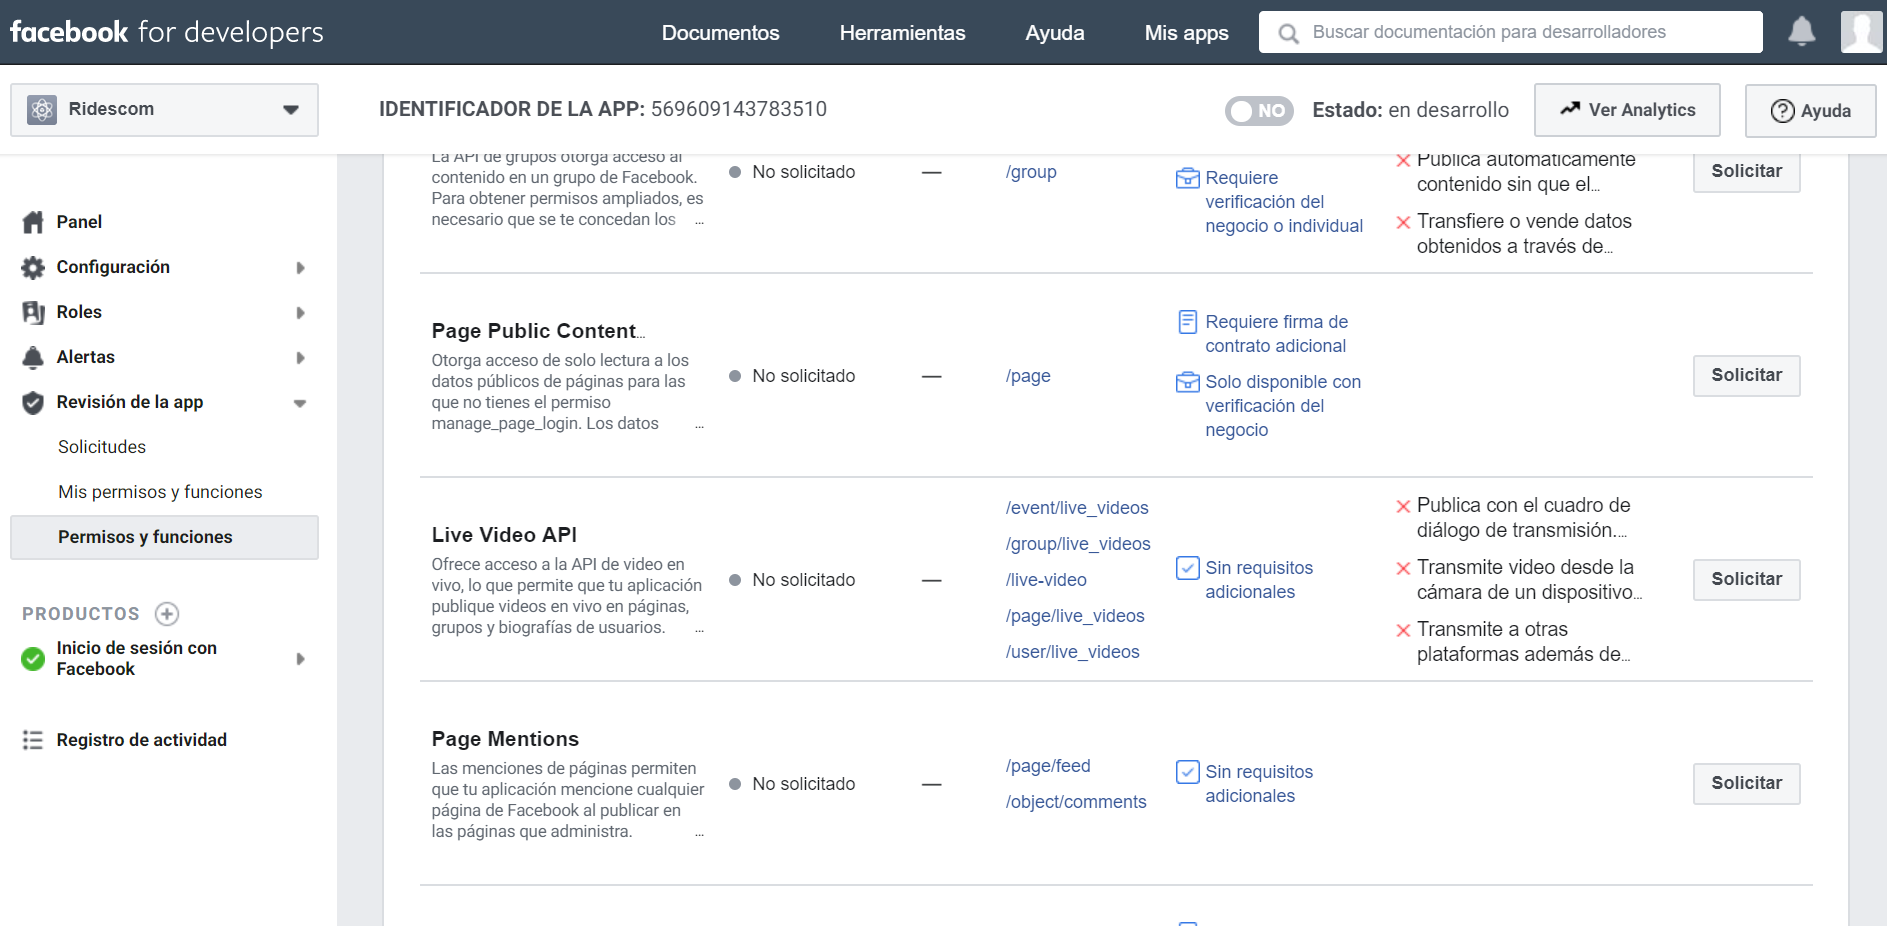
\includegraphics[width=10cm, height=6cm]{Imagenes/FacebookAPI/RequisitoPagina}
		\caption{Requisitos a cumplir para hacer uso de la API de Facebook.}
		\label{requisitosfb}
	\end{figure}
	
	\noindent Dentro de la investigación se encontró que se tenía que seguir paso a paso la
	verificación del negocio y la revisión de la aplicación, con la finalidad de si está todo en orden se
	pueda utilizar las herramientas de Facebook, como se muestra en la siguiente Figura \ref{requisitosfb}. \\
	
	\noindent Realizando la investigación de las actualizaciones para el uso de los plugin de Facebook,
	los datos necesarios para obtener dicha validación, se encontró lo siguiente: \\
	\pagebreak
	
	\textbf{Desarrollo de aplicaciones} \\
	
	En estos documentos, se explica cómo registrar, configurar y desarrollar tu aplicación de modo
	que puedas usar correctamente nuestros productos, API y SDK.
	El ciclo general de desarrollo implica lo siguiente:
	\begin{itemize}
		\item Registrar la aplicación
		\item Seleccionar una situación y agregar productos
		\item Agregar roles
		\item Hacer pruebas en el modo de desarrollo
		\item Solicitar la revisión de aplicaciones
		\item Cambiar al modo activo
	\end{itemize}
	\noindent Repite los pasos Hacer pruebas en el modo de desarrollo y Revisión de
	aplicaciones cada vez que agregues permisos, funciones o productos nuevos o cada vez que
	actualices a una nueva versión de un SDK o de una API.\\
	%https://developers.facebook.com/docs/apps#register
	
	\textbf{Primeros pasos}\\
	Con la API de Pages, las personas pueden actualizar y administrar páginas de Facebook desde su
	aplicación relacionada con la página. Las personas pueden publicar contenido en Facebook o
	Messenger con la identidad de una página. Los casos de uso para API de páginas incluyen:
	\begin{itemize}
		\item Creación de una herramienta de gestión de páginas para clientes o para su
		empresa
		\item Creación de aplicaciones para que los creadores y editores de contenido
		puedan publicar fácilmente como una página
		\item Marketing y publicidad para un negocio utilizando la API de marketing. Para
		obtener más información, consulte API de administración de anuncios y publicaciones de
		páginas no publicadas
		
	\end{itemize}
	%https://developers.facebook.com/docs/pages/getting-started
	
	\textbf{Revisión de apps}\\ 
	
	\noindent Antes de que una app pase a modo activo, es posible que debamos asegurarnos de que
	utilizarás nuestros productos y datos de una manera autorizada. Para lograrlo, requerimos que
	muchas apps se sometan a la revisión de apps.\\
	\noindent En general, el proceso implica especificar el tipo de datos que solicitará la aplicación de
	los usuarios y describir de qué manera utilizará los datos. Según la información que envíes, es
	posible que realicemos un seguimiento y te solicitemos completar otros pasos.\\
	\newline
	¿Cuánto tarda el proceso?\\
	\noindent Por lo general, nos lleva menos de una semana procesar un envío y, con frecuencia, solo
	2 o 3 días. Sin embargo, es posible que tardemos más en períodos pico. Debes tener en cuenta
	que, debido a cambios recientes en el proceso de revisión y al alto volumen de envíos, es posible
	que tardemos varias semanas para completar el proceso de revisión de las apps enviadas.\\
	\newline
	Verificación adicional \\
	\noindent Después de enviar la aplicación para su revisión, es posible que verifiquemos tu	identidad como empresa o como persona. Para hacerlo, te enviaremos una alerta a la bandeja de
	entrada del panel de aplicaciones. La alerta incluirá un enlace para comenzar el proceso de	verificación.\\ %https://developers.facebook.com/docs/apps/review/#supplemental-terms
	
	\noindent Con lo antes investigado se siguió el proceso para verificar la verificación del negocio y
	la comprobación de la aplicación, como se muestra en la siguiente Figura \ref{creacionFB}.
	\pagebreak
	
	\begin{figure}[hbt!]
		\centering
		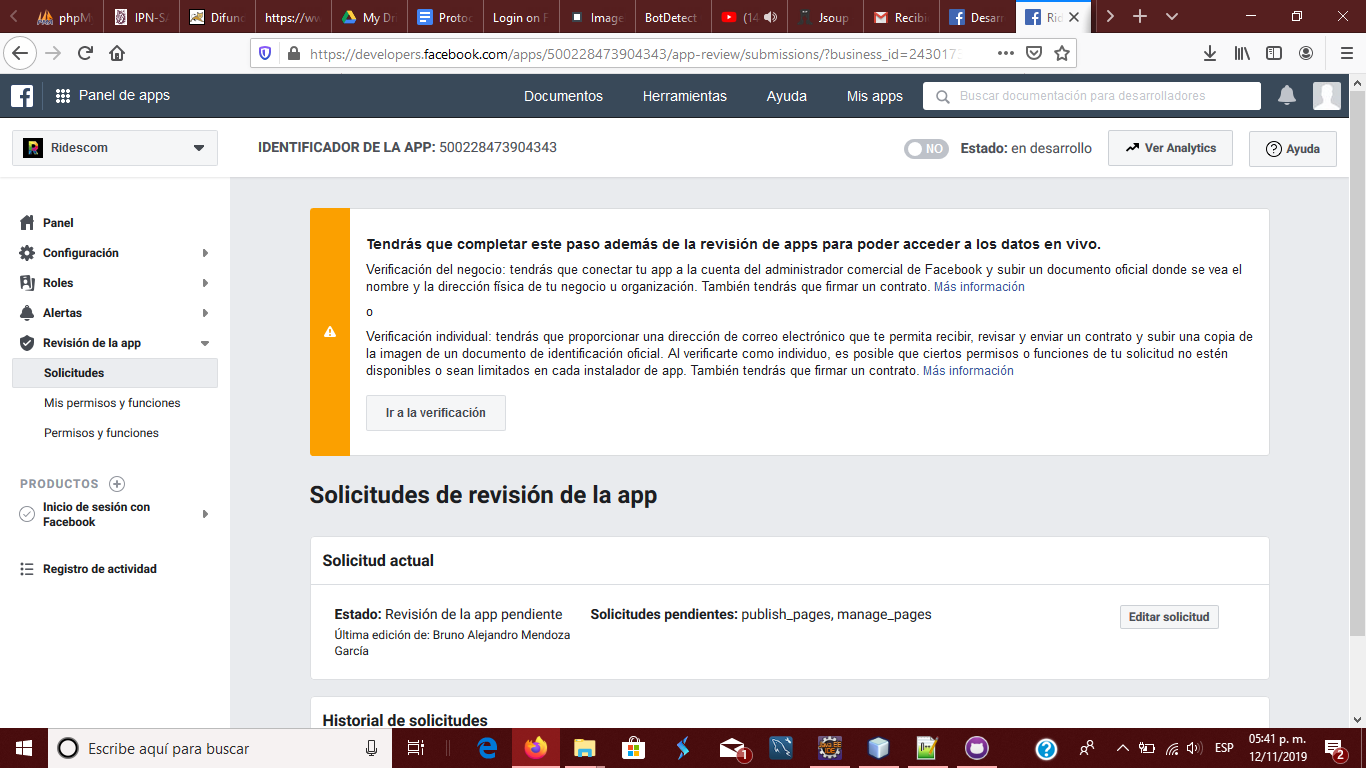
\includegraphics[width=15cm, height=6cm]{Imagenes/FacebookAPI/Facebook1}
		\caption{Solicitud de revisión de app.}
		\label{creacionFB}
	\end{figure}

	\noindent En la Figura \ref{creacionFB2} se muestran los datos necesarios a validar para poder hacer uso del API de Facebook. Especifícamente, la de interés para el proyecto es el API de publish pages.
	\begin{figure}[hbt!]
		\centering
		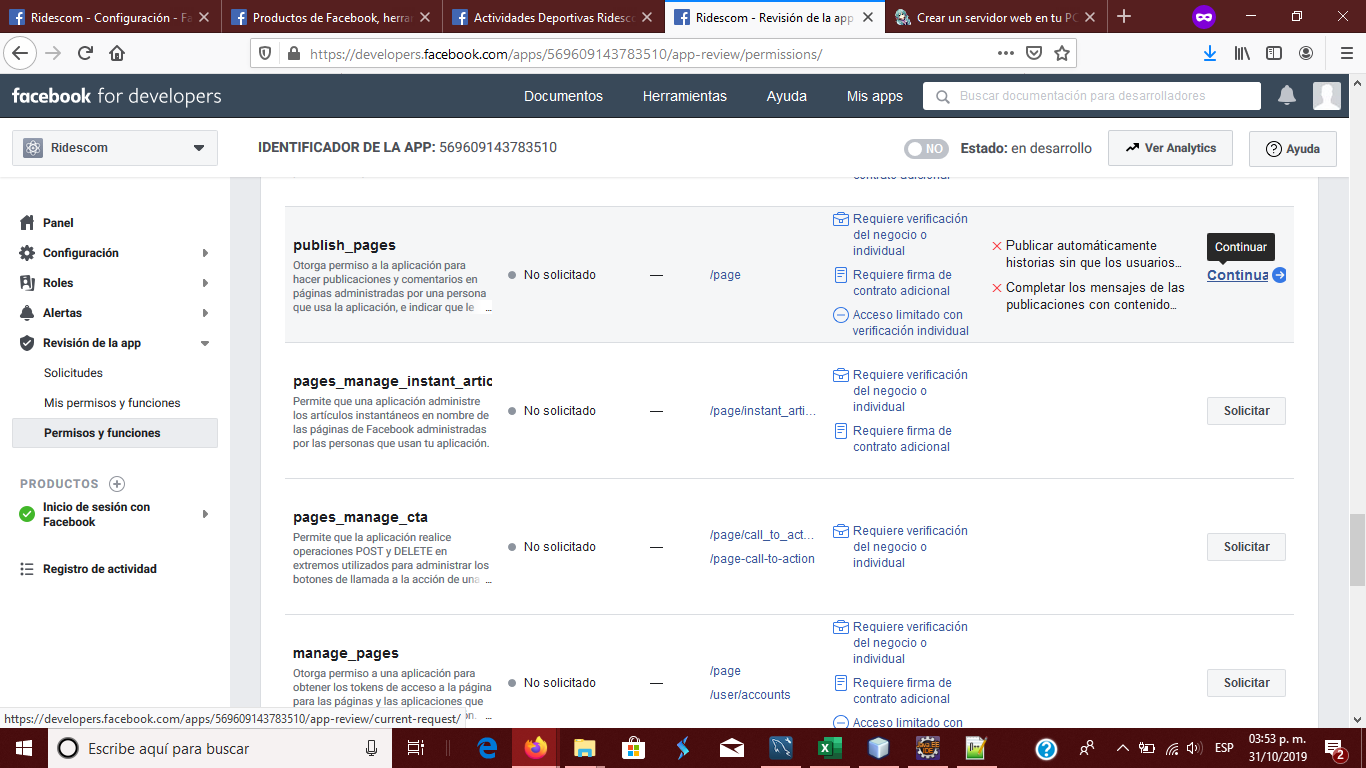
\includegraphics[width=15cm, height=6cm]{Imagenes/FacebookAPI/Facebook2}
		\caption{Datos a verificar.}
		\label{creacionFB2}
	\end{figure}

	\noindent En la Figura \ref{creacionFB3} se muestra los campos requeridos para poder hacer la solicitud de revisión de la aplicación. Como se puede observar se solicita un icono que identifique a la aplicación, a su vez se solicita una URL en la que se específique las políticas de privacidad, ya que se hace uso de manejo de información personal.
\pagebreak
	\begin{figure}[hbt!]
		\centering
		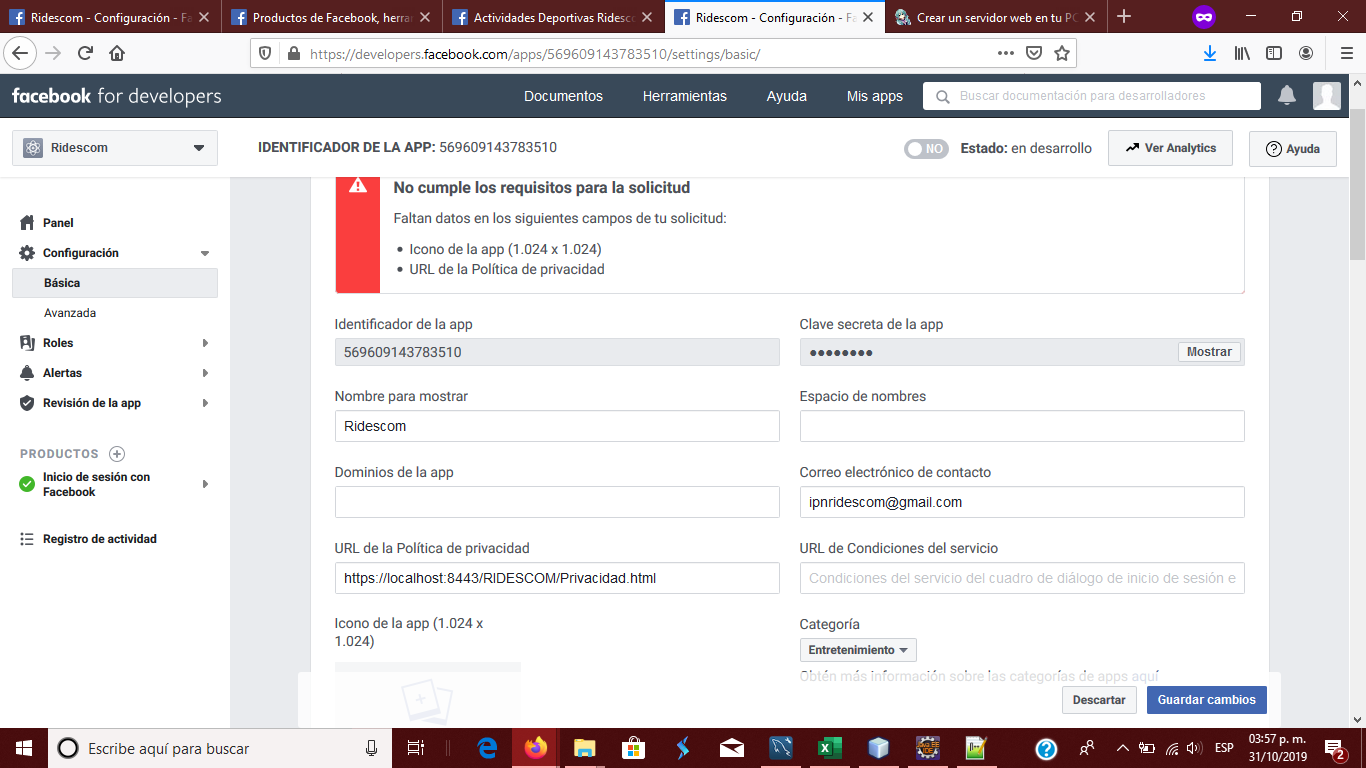
\includegraphics[width=15cm, height=6cm]{Imagenes/FacebookAPI/Facebook3}
		\caption{Solicitud de datos para revisión de la aplicación.}
		\label{creacionFB3}
	\end{figure}

	\noindent Al ingresar a ver la configuración de la aplicación, en el apartado de solicitudes podemos ver el estatus actual de la solicitud realizada, como se puede apreciar en la Figura \ref{creacionFB7}.

	\begin{figure}[hbt!]
		\centering
		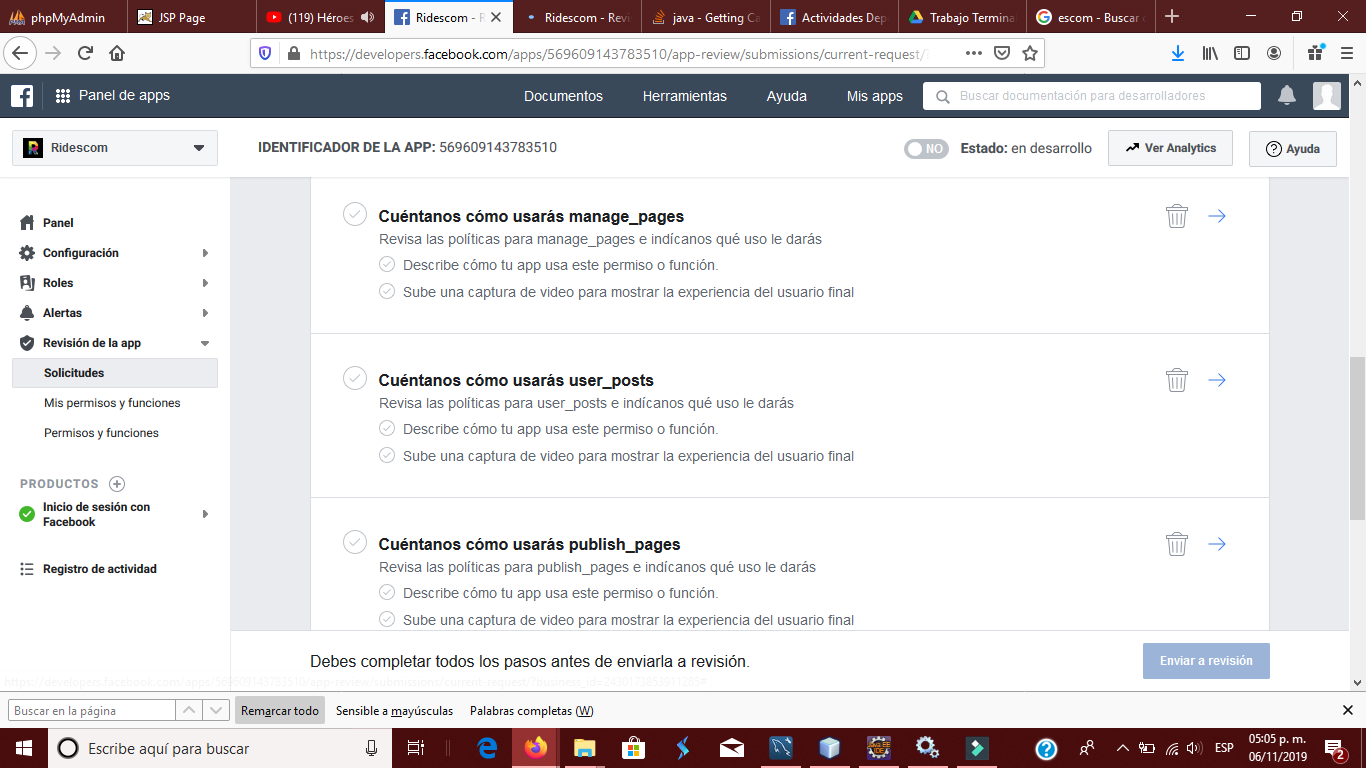
\includegraphics[width=15cm, height=6cm]{Imagenes/FacebookAPI/Facebook7}
		\caption{Estatus de solicitudes.}
		\label{creacionFB7}
	\end{figure}
	
	\noindent En la Figura \ref{creacionFB4} se da una breve descripción de la finalidad de la integración de la API de Facebook en el proyecto desarrollando.
\pagebreak
	\begin{figure}[hbt!]
		\centering
		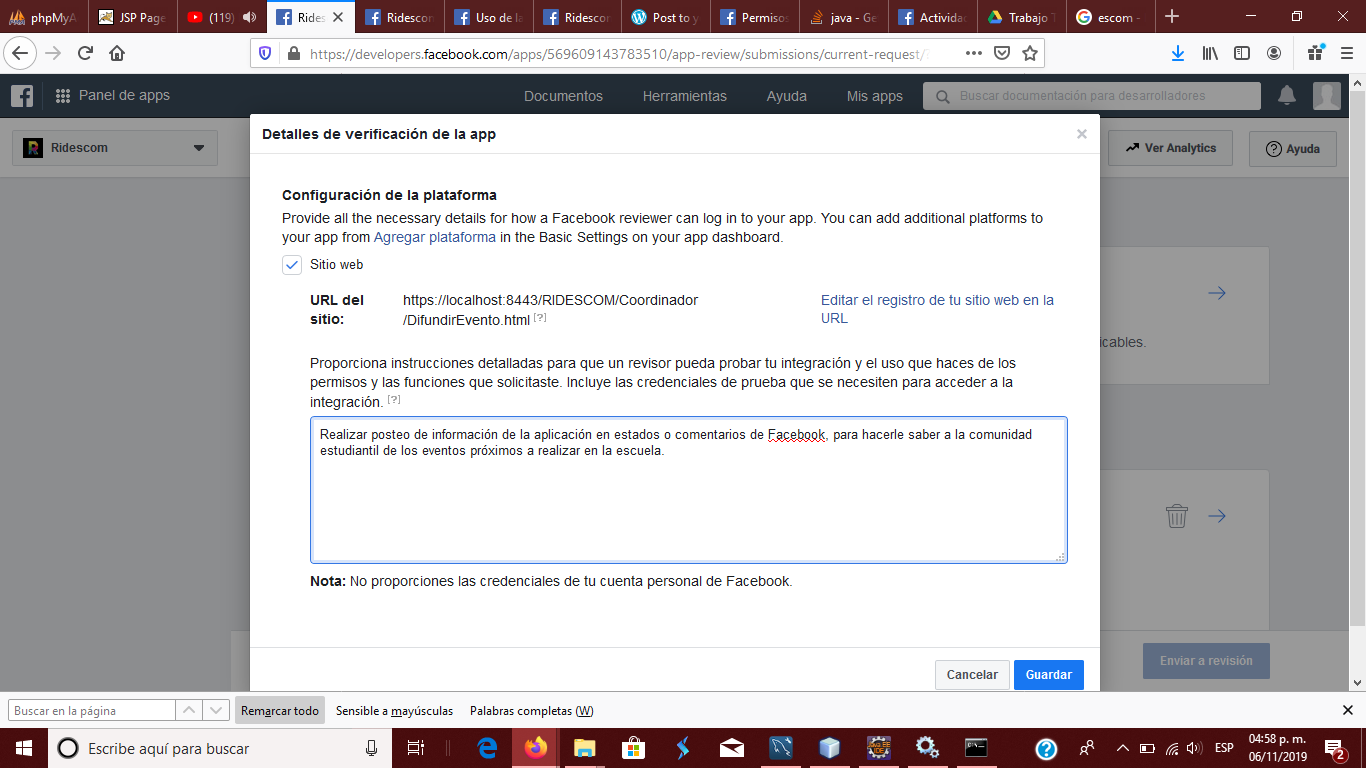
\includegraphics[width=15cm, height=6cm]{Imagenes/FacebookAPI/Facebook4}
		\caption{Descripción de la finalidad de la aplicación.}
		\label{creacionFB4}
	\end{figure}

	\noindent Como complemento a la solicitud, en la Figura \ref{creacionFB5} se da una breve descripción de la finalidad de la solicitud manage pages.

	\begin{figure}[hbt!]
		\centering
		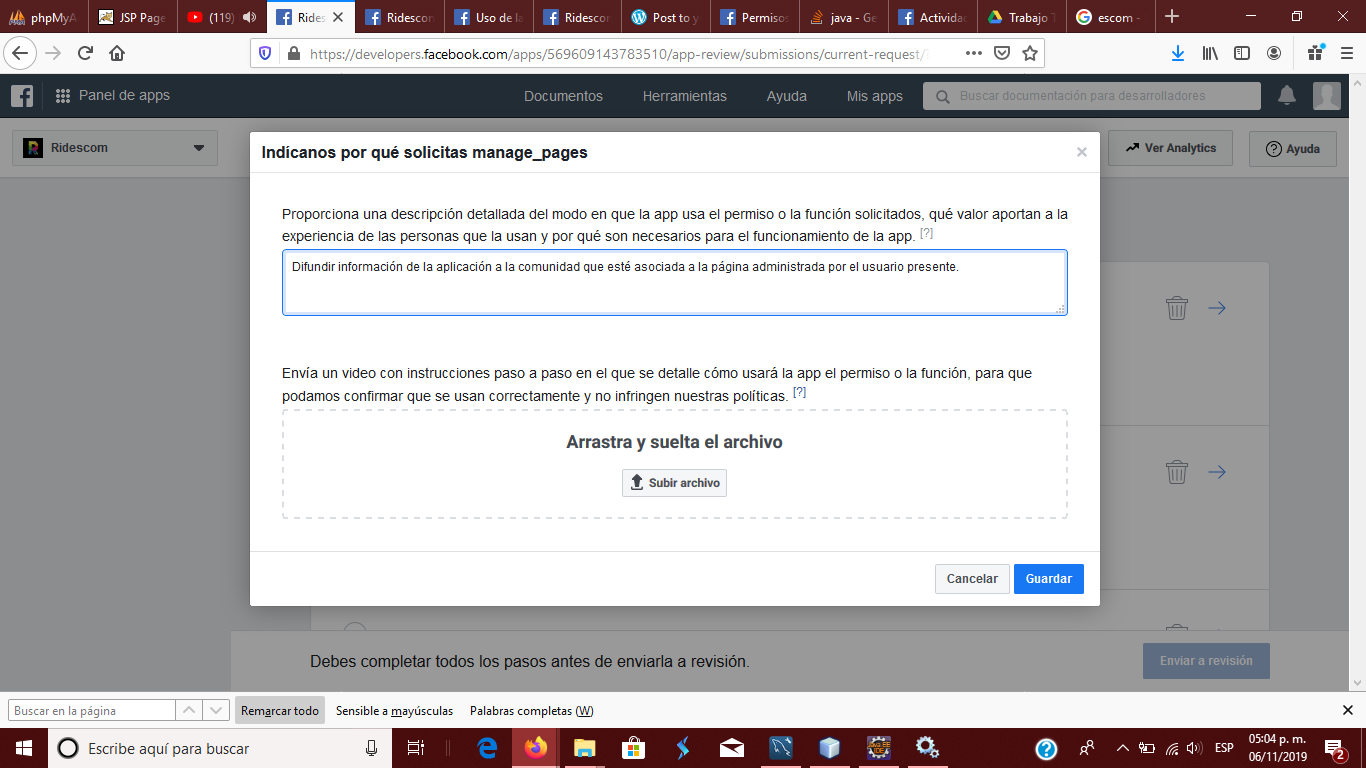
\includegraphics[width=15cm, height=6cm]{Imagenes/FacebookAPI/Facebook5}
		\caption{Descripción del uso de manage page en la aplicación desarrollando.}
		\label{creacionFB5}
	\end{figure}

	\noindent Al completar los campos requeridos nos muestra un mensaje de confirmación de la solicitud de revisión, como se muestra en la Figura \ref{creacionFB15}
\pagebreak
	\begin{figure}[hbt!]
		\centering
		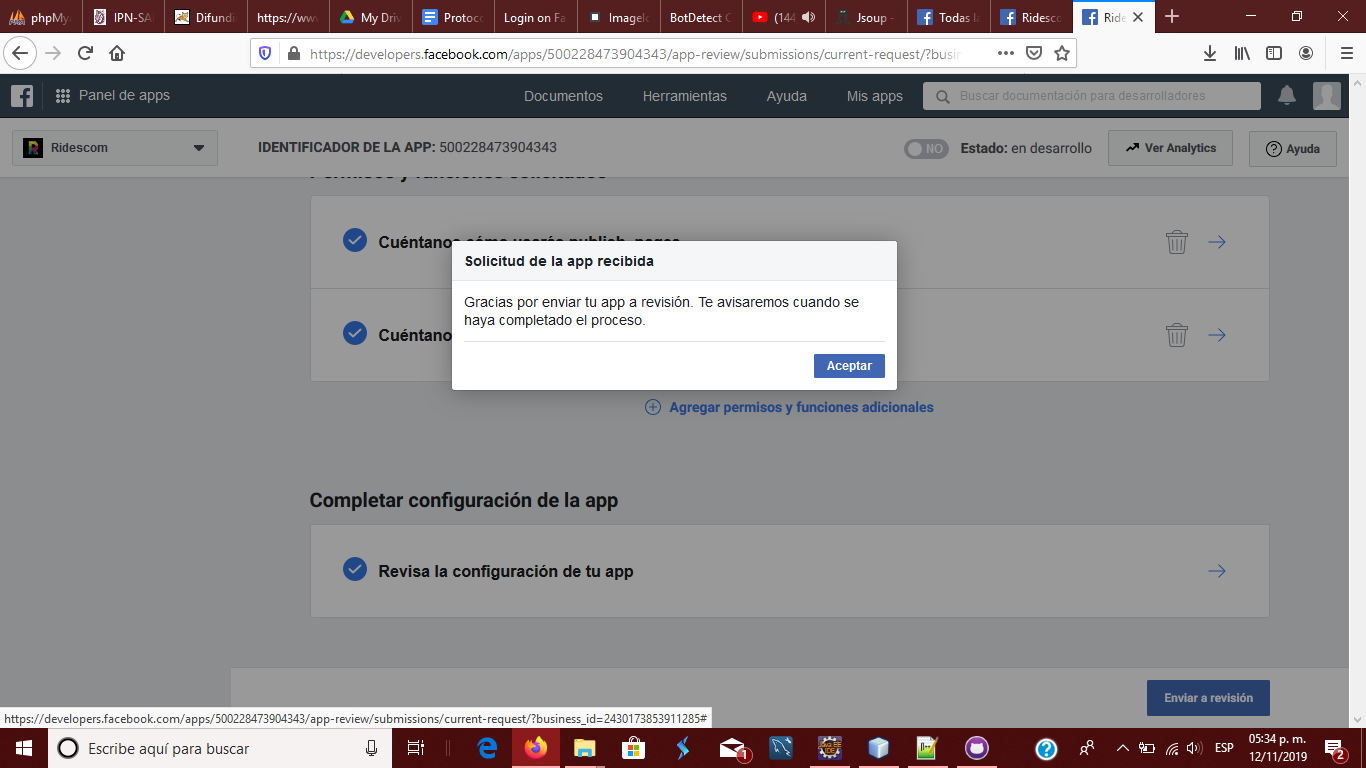
\includegraphics[width=15cm, height=6cm]{Imagenes/FacebookAPI/Facebook15}
		\caption{paso 15}
		\label{creacionFB15}
	\end{figure}

	\noindent Una vez completado los pasos anteriores, nos es re dirigido a la página donde se visualizan las aplicaciones que se tienen, como se puede ver en la Figura \ref{creacionFB6}.
	\begin{figure}[hbt!]
		\centering
		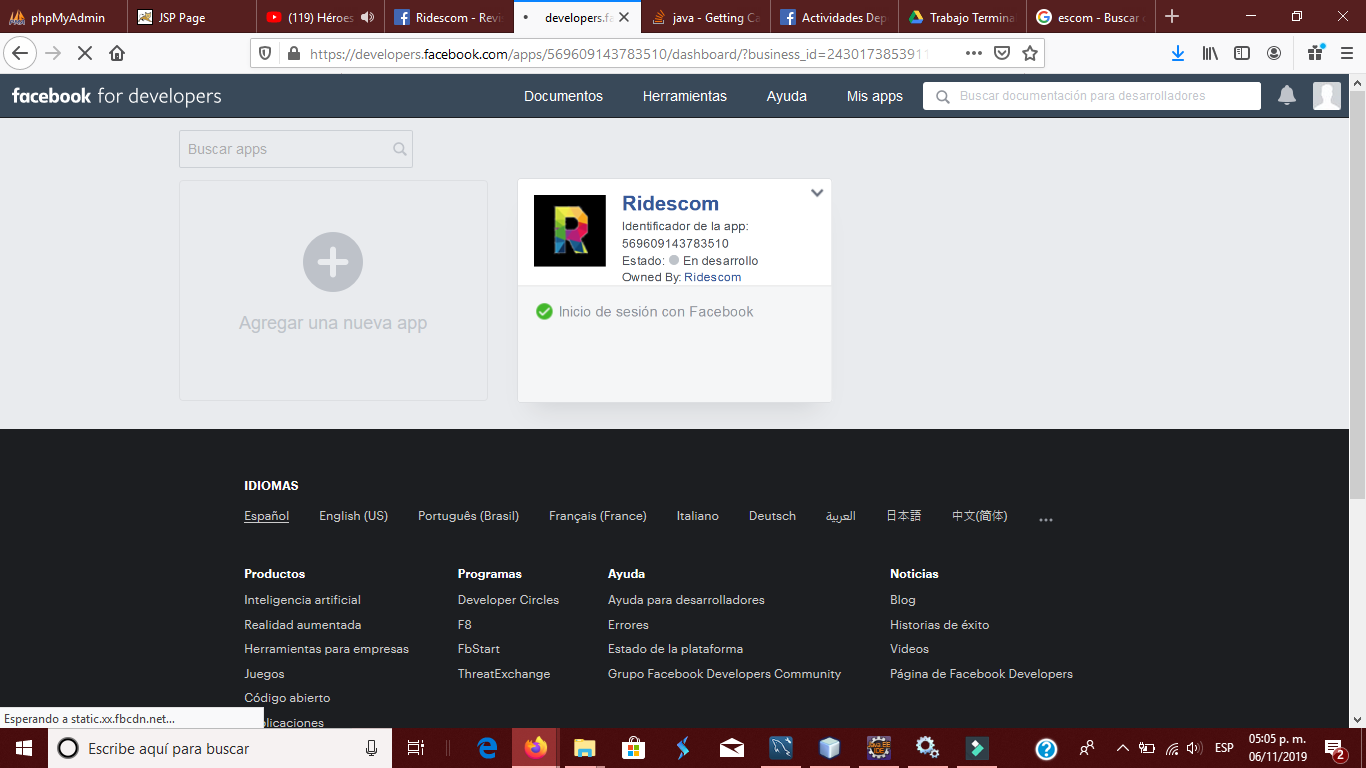
\includegraphics[width=15cm, height=6cm]{Imagenes/FacebookAPI/Facebook6}
		\caption{Solicitud completada}
		\label{creacionFB6}
	\end{figure}
	
	\noindent En la Figura \ref{creacionFB8}, se puede visualizar la configuración actual de la aplicación. De tal manera que se visualiza que no existe algún dato faltante.

	\begin{figure}[hbt!]
		\centering
		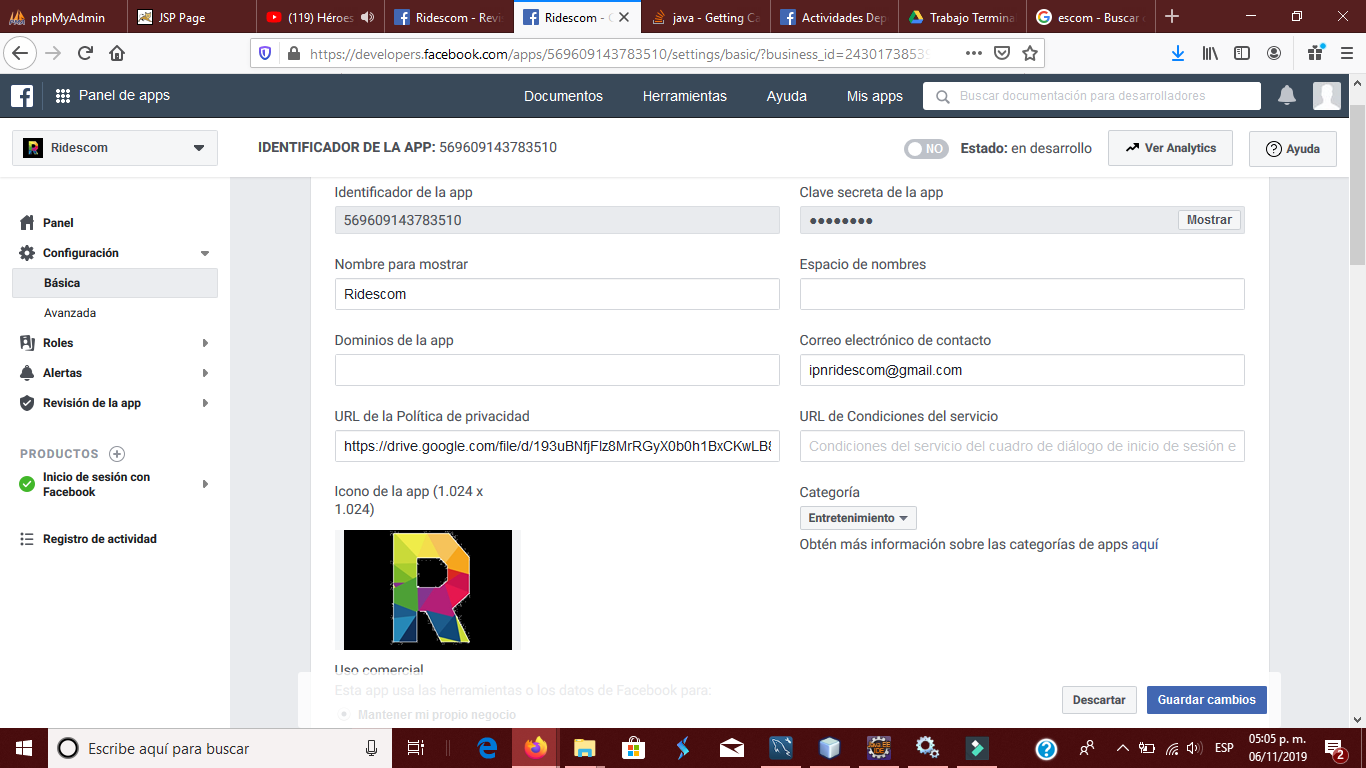
\includegraphics[width=15cm, height=6cm]{Imagenes/FacebookAPI/Facebook8}
		\caption{Configuración de la aplicación.}
		\label{creacionFB8}
	\end{figure}
\pagebreak
	
	En la Figura \ref{creacionFB9}, se puede observar el estatus de la solicitud de la información individual. En esta se solicitó información acerca de la persona que estaba desarrollando la aplicación.
	\begin{figure}[hbt!]
		\centering
		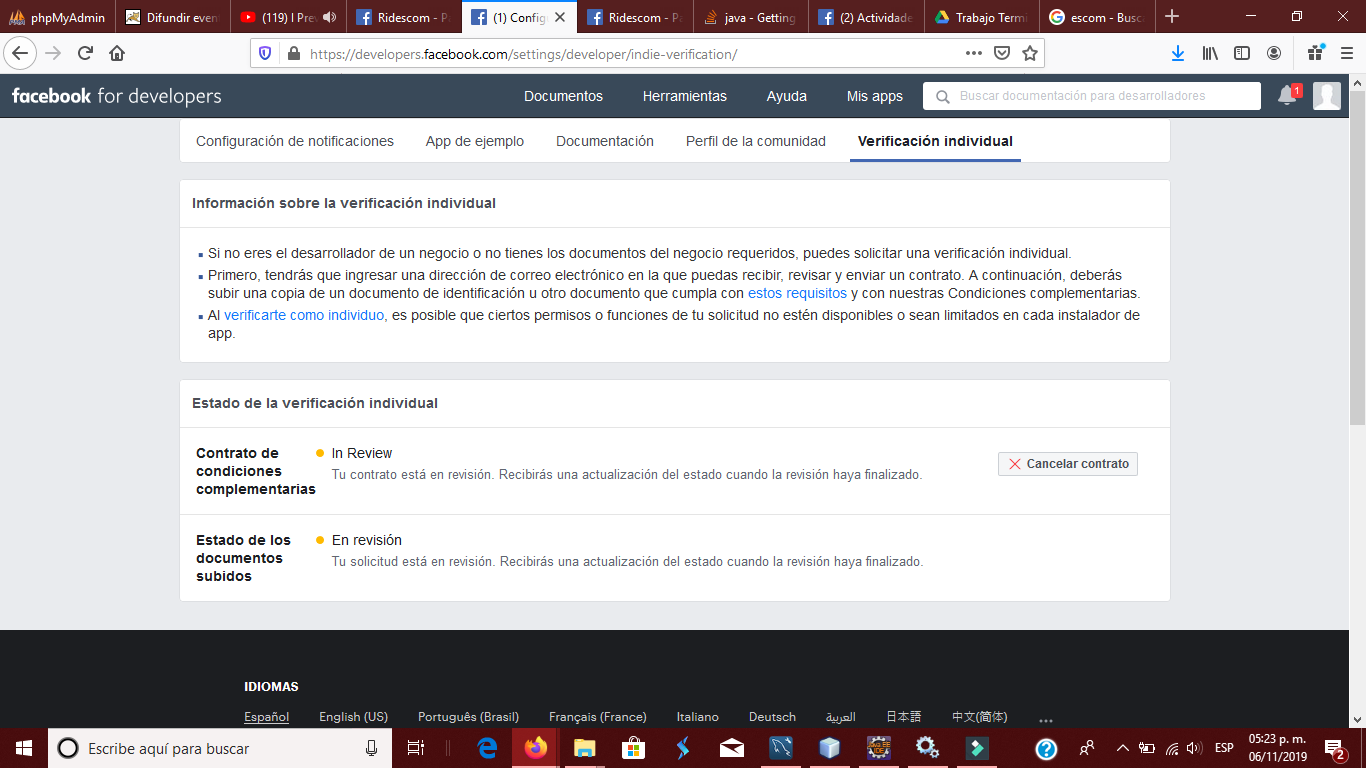
\includegraphics[width=15cm, height=6cm]{Imagenes/FacebookAPI/Facebook9}
		\caption{Estatus solicitud individual.}
		\label{creacionFB9}
	\end{figure}

	En la Figura \ref{creacionFB11}, se puede observar el estatus de la verificación del negocio. En este se solicitaron datos acerca de la empresa para la cual se estaba creando el proyecto, que en nuestro caso se envió la información acerca del Trabajo Terminal.
	\begin{figure}[hbt!]
		\centering
		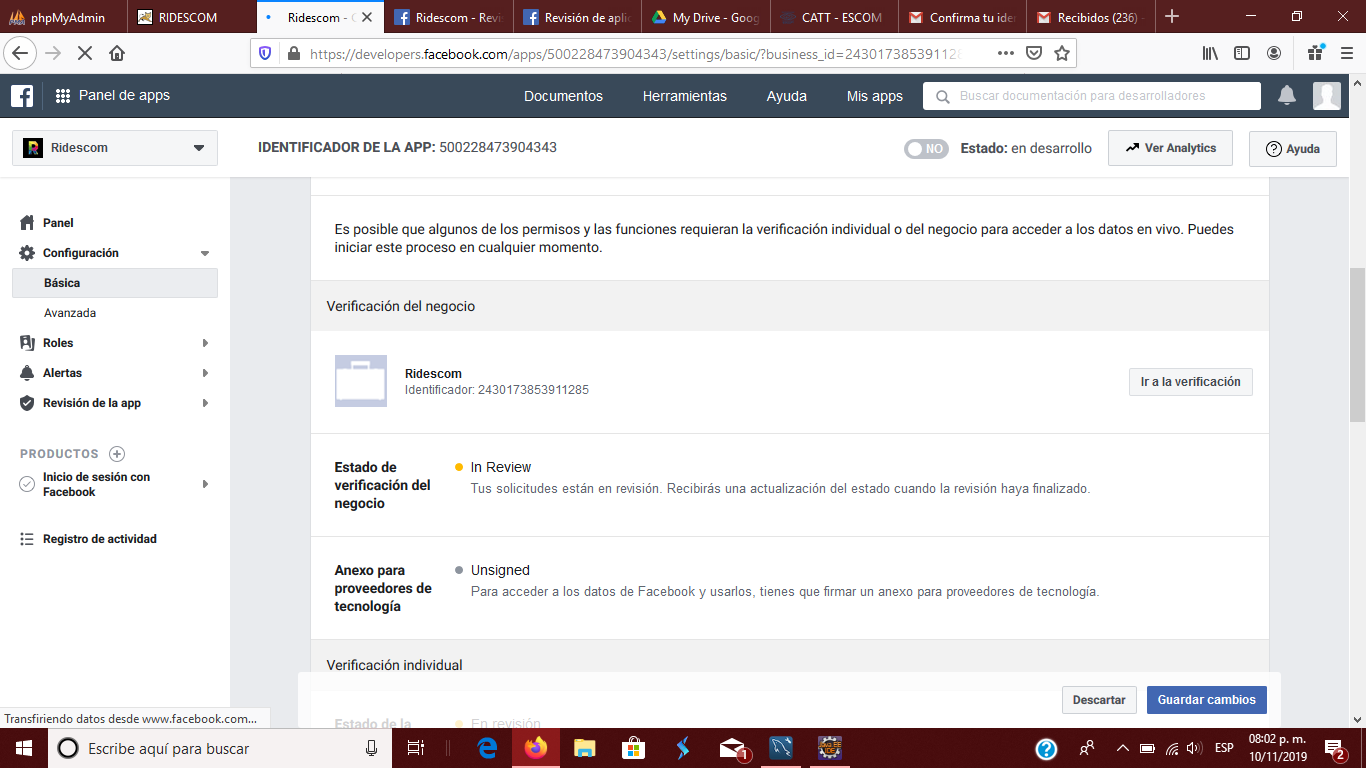
\includegraphics[width=15cm, height=6cm]{Imagenes/FacebookAPI/Facebook11}
		\caption{Estatus Solicitud Negocio.}
		\label{creacionFB11}
	\end{figure}
\pagebreak
	Al terminar de revisar el estatus individual de cada requisito, se muestra de manera gráfica el proceso actual de la o las solicitudes realizadas. En está se puede apreciar que el tiempo estimado en la que se proporcionaría una respuesta es en 5 días, como se muestra en la Figura \ref{creacionFB12}.

	\begin{figure}[hbt!]
		\centering
		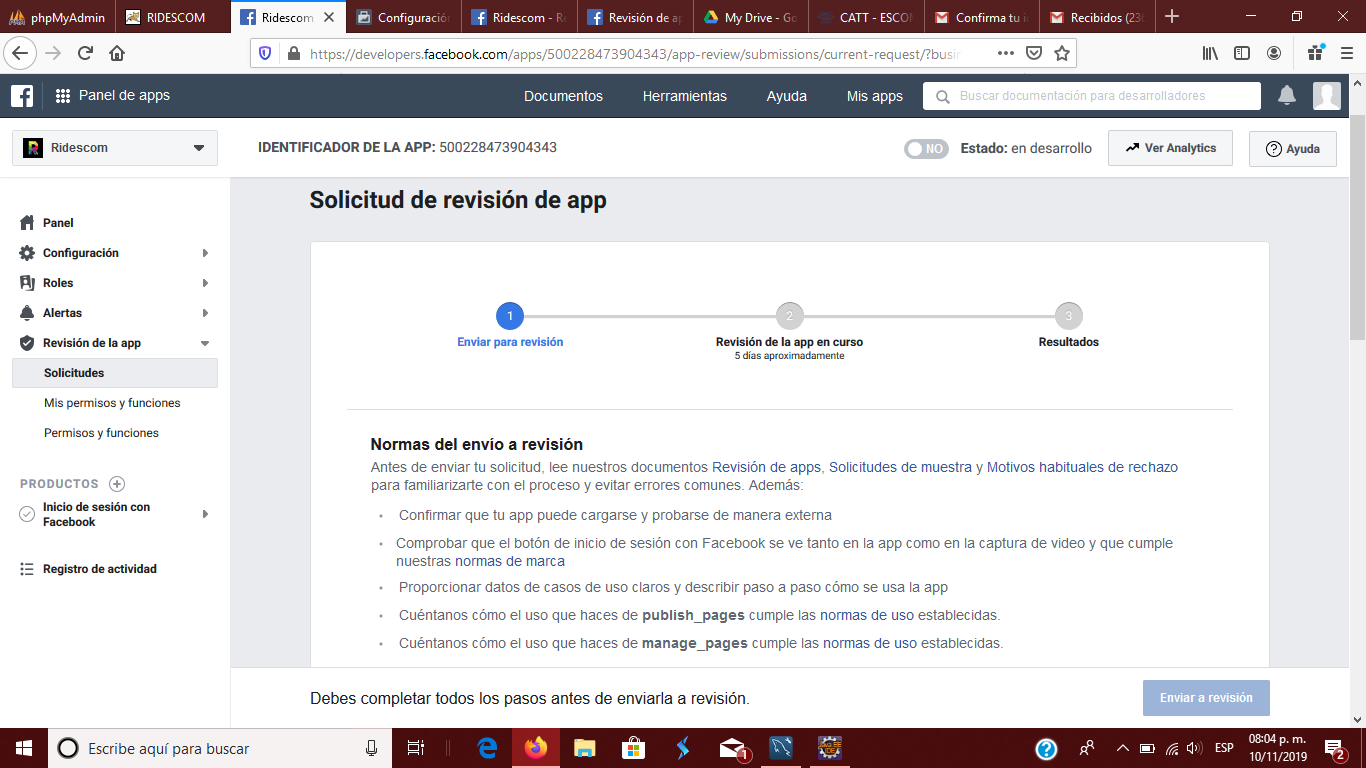
\includegraphics[width=15cm, height=6cm]{Imagenes/FacebookAPI/Facebook12}
		\caption{Gráfica de estatus de solicitud.}
		\label{creacionFB12}
	\end{figure}
\pagebreak
	\noindent Al pasar los 5 días en los que se revisaba la solicitud, se notifica que es requisito el enviar datos mucho más especifícos del negocio u organización, como se muestra en la Figura \ref{creacionFB16}. Siendo en este primer punto un factor de incertidumbre ya que al tratarse de un proyecto escolar, el envío de estos datos pueda repercutir en temas mucho más sencibles.

	\begin{figure}[hbt!]
		\centering
		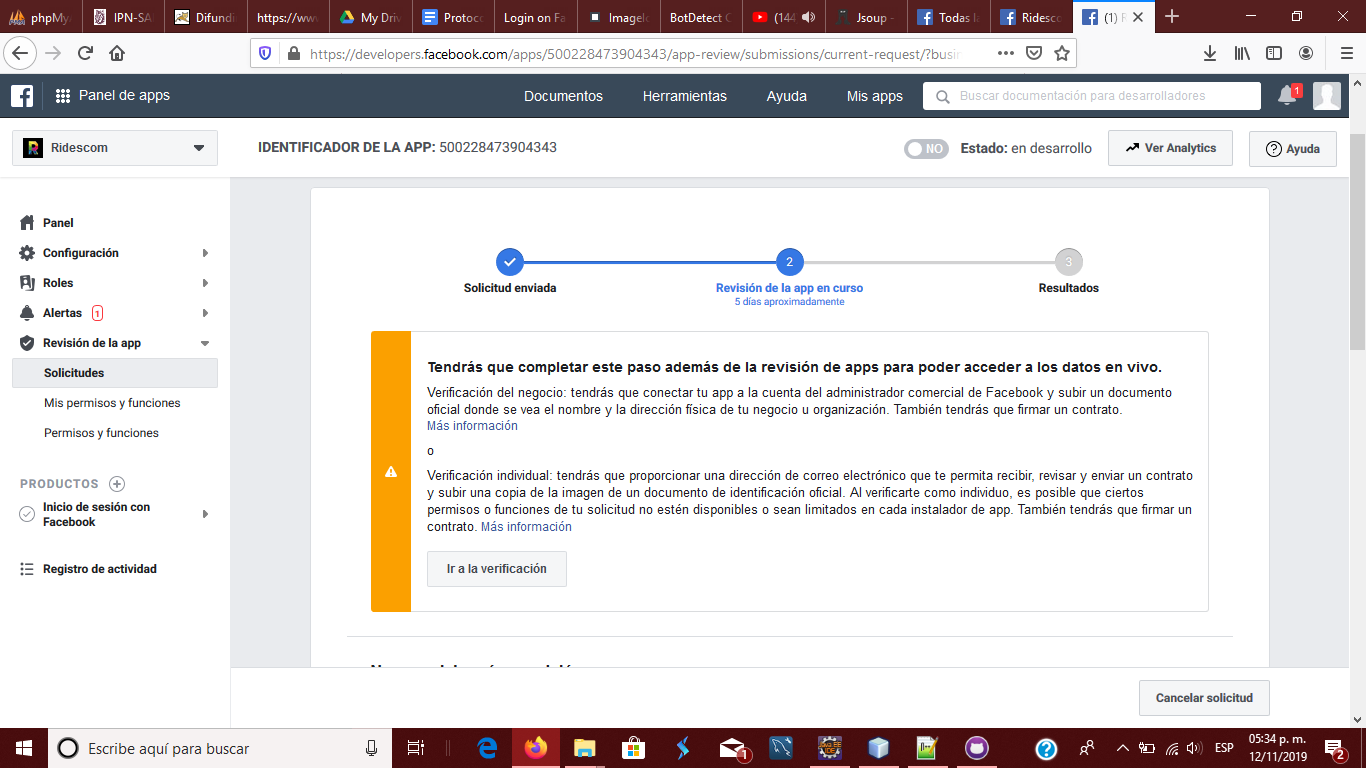
\includegraphics[width=15cm, height=6cm]{Imagenes/FacebookAPI/Facebook16}
		\caption{Respuesta a solititud.}
		\label{creacionFB16}
	\end{figure}
	
	
	\chapter{Apartado G: Base de Datos}
	\noindent En este apartado, se muestra la estructura de la base de datos que tiene la aplicación web. Se tomó en consideración los requisitos y problemática que se tenían para proporcionar una respuesta óptima de los datos. Cabe mencionar que la base de datos se modeló para que esta pueda funcionar cuando al proyecto se agreguen más unidades académicas.
	
		\label{BasedeDatos}
		\begin{figure}[hbt!]
			\centering
			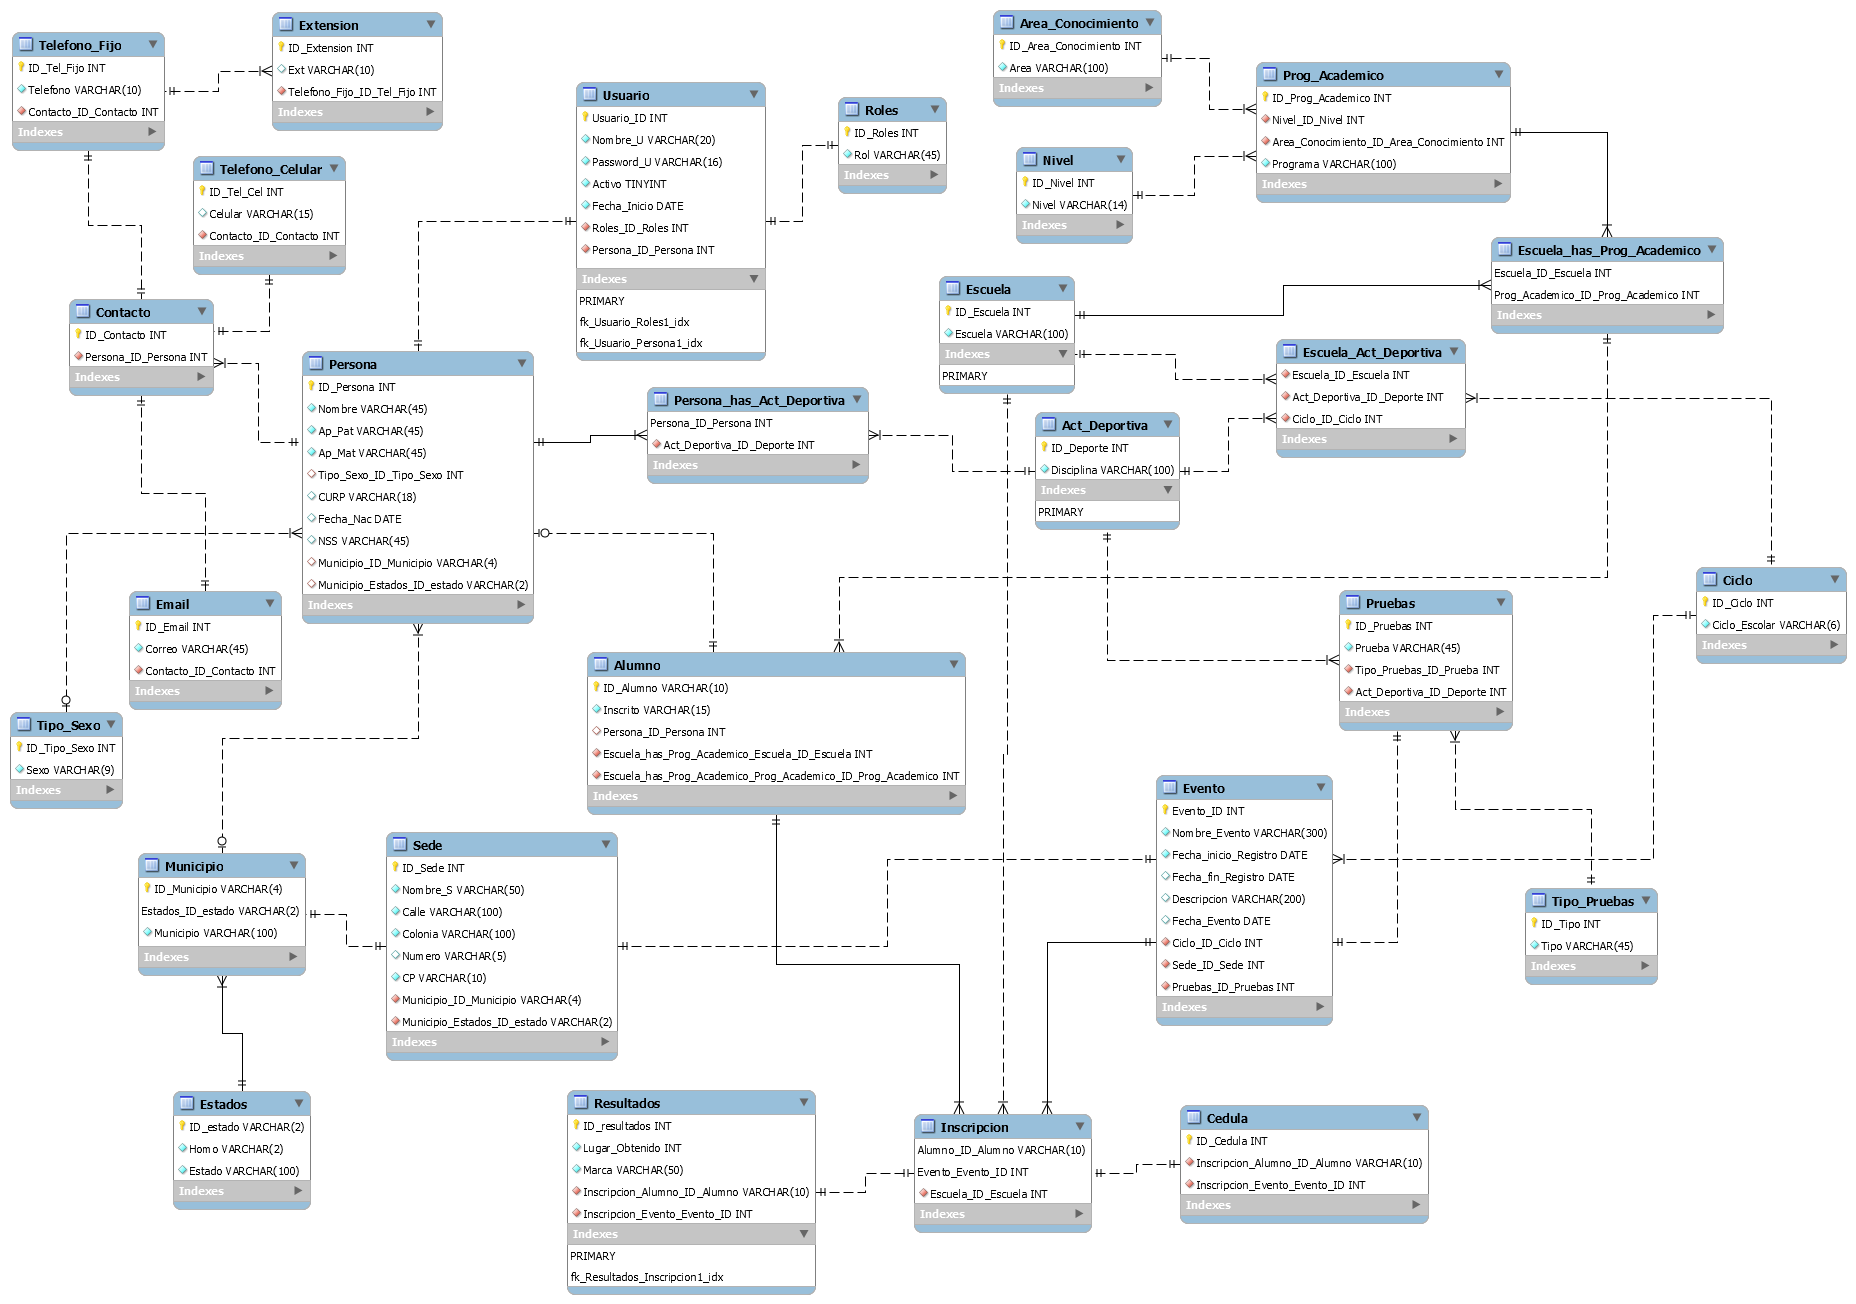
\includegraphics[angle=90, width=14cm, height=19cm]{Imagenes/RIDESCOM.png}
			\caption{Estructura de la Base de Datos de RIDESCOM}
			\label{BaseDatos}
		\end{figure}
		
		
	
	\pagebreak
		
